\documentclass[11pt,a4paper]{article}

\usepackage[margin=2.2cm]{geometry}
\usepackage{hyperref}
\usepackage{enumitem}
\usepackage{listings}
\usepackage{xcolor}
\usepackage{booktabs}
\usepackage{titlesec}
\usepackage[T1]{fontenc}
\usepackage{lmodern}
\usepackage{parskip}
\usepackage{graphicx}
\usepackage{array}
\usepackage{tabularx}
\usepackage{colortbl}
\usepackage{longtable}
\usepackage{fancyhdr}
\usepackage{microtype}
\usepackage{tikz}
\usetikzlibrary{shapes.geometric,arrows.meta,positioning,fit,backgrounds,calc}

% Prevent overfull hboxes for long inline code
\setlength{\emergencystretch}{3em}
\hbadness=10000  % suppress underfull warnings

% ── Colors ───────────────────────────────────────────────────────────────────
\definecolor{headerblue}{RGB}{21,101,192}
\definecolor{subheadteal}{RGB}{2,119,189}
\definecolor{delivercolor}{RGB}{2,136,209}
\definecolor{tblheader}{RGB}{21,101,192}
\definecolor{tblrowalt}{RGB}{227,242,253}
\definecolor{tblrowwhite}{RGB}{255,255,255}
\definecolor{linkblue}{RGB}{21,101,192}
% Stretch goals / callout colors
\definecolor{stretchbg}{RGB}{255,248,225}
\definecolor{stretchborder}{RGB}{230,162,30}
% Code block colors (GitHub light theme)
\definecolor{codebg}{RGB}{246,248,250}
\definecolor{codeborder}{RGB}{208,215,222}
\definecolor{codefg}{RGB}{36,41,47}
\definecolor{codekw}{RGB}{0,82,185}
\definecolor{codestr}{RGB}{10,75,105}
\definecolor{codecomment}{RGB}{110,119,129}
\definecolor{codetype}{RGB}{111,66,193}

\hypersetup{
    colorlinks=true,
    linkcolor=linkblue,
    urlcolor=linkblue,
    citecolor=linkblue,
    pdftitle={GSoC 2026 Application -- Open Responses \& Generative UI for API Dash},
    pdfauthor={Shridhar Panigrahi},
}

% ── Code style (GitHub light) ─────────────────────────────────────────────────
\lstdefinestyle{darkcode}{
    basicstyle=\ttfamily\small\color{codefg},
    backgroundcolor=\color{codebg},
    keywordstyle=\color{codekw}\bfseries,
    stringstyle=\color{codestr},
    commentstyle=\color{codecomment}\itshape,
    showstringspaces=false,
    breaklines=true,
    frame=single,
    framesep=8pt,
    rulecolor=\color{codeborder},
    xleftmargin=8pt,
    xrightmargin=8pt,
    aboveskip=8pt,
    belowskip=8pt,
    numbers=none,
    morekeywords={sealed,class,factory,return,switch,const,String,Map,dynamic,bool,void,final,List,int},
}

\lstdefinestyle{jsoncode}{
    basicstyle=\ttfamily\small\color{codefg},
    backgroundcolor=\color{codebg},
    showstringspaces=false,
    breaklines=true,
    frame=single,
    framesep=8pt,
    rulecolor=\color{codeborder},
    xleftmargin=8pt,
    xrightmargin=8pt,
    aboveskip=8pt,
    belowskip=8pt,
    numbers=none,
}

% ── Section formatting ────────────────────────────────────────────────────────
\titleformat{\section}
  {\large\bfseries}{}{0pt}{}
  [\vspace{2pt}\textcolor{headerblue}{\rule{\textwidth}{1.5pt}}]

\titleformat{\subsection}
  {\normalsize\bfseries\color{subheadteal}}{}{0pt}{}

\titleformat{\subsubsection}
  {\normalsize\bfseries\color{subheadteal}}{}{0pt}{}

\titlespacing{\section}{0pt}{12pt}{6pt}
\titlespacing{\subsection}{0pt}{8pt}{4pt}
\titlespacing{\subsubsection}{0pt}{6pt}{3pt}

\setlist[itemize]{topsep=3pt,itemsep=2pt,parsep=1pt,leftmargin=1.8em}
\setlist[enumerate]{topsep=3pt,itemsep=2pt,parsep=1pt,leftmargin=1.8em}

% ── Header / Footer ───────────────────────────────────────────────────────────
\pagestyle{fancy}
\fancyhf{}
\renewcommand{\headrulewidth}{0pt}
\fancyhead[C]{\small\color{gray}GSoC 2026 -- Shridhar Panigrahi -- Open Responses \& Generative UI}
\fancyfoot[C]{\small Page \thepage/\pageref{docendpage}}
\fancypagestyle{plain}{
  \fancyhf{}
  \renewcommand{\headrulewidth}{0pt}
  \fancyfoot[C]{\small Page \thepage/\pageref{docendpage}}
}

% ── Helpers ───────────────────────────────────────────────────────────────────
\newcommand{\deliverable}[1]{%
  \vspace{6pt}%
  \noindent{\setlength{\fboxsep}{8pt}%
  \colorbox{tblrowalt}{%
    \parbox{\dimexpr\linewidth-2\fboxsep\relax}{%
      \vspace{2pt}%
      {\small\textcolor{headerblue}{\bfseries Deliverable:} \textcolor{subheadteal}{\itshape #1}}%
      \vspace{2pt}%
    }%
  }}%
  \vspace{6pt}%
}

\begin{document}

% ══════════════════════════════════════════════════════════════════════════════
%  COVER PAGE
% ══════════════════════════════════════════════════════════════════════════════
\thispagestyle{plain}
\begin{center}
  \includegraphics[width=0.18\textwidth]{macos/Runner/Assets.xcassets/AppIcon.appiconset/app_icon_1024.png}\\[14pt]
  {\LARGE\bfseries GSoC 2026 Application}\\[8pt]
  {\large Open Responses Protocol Support \&\\[4pt]
         Generative UI Rendering Engine\\[4pt]
         for API Dash}\\[20pt]
  \textcolor{headerblue}{\rule{0.6\textwidth}{1pt}}\\[20pt]
  {\large\bfseries Shridhar Panigrahi}\\[8pt]
  \href{mailto:sridharpanigrahi2006@gmail.com}{sridharpanigrahi2006@gmail.com}\\[3pt]
  \href{https://github.com/sridhar-panigrahi}{github.com/sridhar-panigrahi}\\[3pt]
  \href{https://www.linkedin.com/in/shridhar-panigrahi-8bb176362}{linkedin.com/in/shridhar-panigrahi-8bb176362}\\[16pt]
  Polaris School of Technology, Bangalore\\[3pt]
  B.Tech Computer Science (AI \& ML) \textbar{} 1st Year \textbar{} Expected 2029\\[3pt]
  IST (UTC+5:30)
\end{center}

\newpage

% ══════════════════════════════════════════════════════════════════════════════
%  CONTACT INFORMATION
% ══════════════════════════════════════════════════════════════════════════════
\section{Name and Contact Information}

\begin{tabular}{@{}p{3.2cm} p{10cm}@{}}
  \textbf{Name:}        & Shridhar Panigrahi \\[3pt]
  \textbf{Email:}       & \href{mailto:sridharpanigrahi2006@gmail.com}{sridharpanigrahi2006@gmail.com} \\[3pt]
  \textbf{GitHub:}      & \href{https://github.com/sridhar-panigrahi}{sridhar-panigrahi} \\[3pt]
  \textbf{LinkedIn:}    & \href{https://www.linkedin.com/in/shridhar-panigrahi-8bb176362}{shridhar-panigrahi-8bb176362} \\[3pt]
  \textbf{Time zone:}   & IST (UTC+5:30) \\[3pt]
  \textbf{University:}  & Polaris School of Technology, Bangalore \\[3pt]
  \textbf{Program:}     & B.Tech CSE (AI \& ML), 1st Year \\[3pt]
  \textbf{Graduation:}  & Expected 2029 \\
\end{tabular}

% ══════════════════════════════════════════════════════════════════════════════
%  MOTIVATION & PAST EXPERIENCE
% ══════════════════════════════════════════════════════════════════════════════
\section{Motivation \& Past Experience}

\subsection{1. Have you worked on or contributed to a FOSS project before?}

Yes. I have \textcolor{headerblue}{\bfseries 11 merged PRs} across \textcolor{headerblue}{\bfseries 5 open-source projects}. API Dash is the project I've been focused on for GSoC, but I've also contributed to large codebases in Python, Java, Go, and Rust:

\begin{itemize}
  \item \textbf{astropy} -- 3 merged PRs
    (\href{https://github.com/astropy/astropy/pull/19403}{\#19403},
     \href{https://github.com/astropy/astropy/pull/19404}{\#19404},
     \href{https://github.com/astropy/astropy/pull/19450}{\#19450}):
    Fixed an f-string bug, silent data corruption in \texttt{FITS\_rec}, and table index corruption on failed row assignment. \textcolor{headerblue}{\bfseries 500k+} line Python codebase.

  \item \textbf{Hyperledger Besu} -- 4 merged PRs
    (\href{https://github.com/hyperledger/besu/pull/10020}{\#10020},
     \href{https://github.com/hyperledger/besu/pull/10042}{\#10042},
     \href{https://github.com/hyperledger/besu/pull/10051}{\#10051},
     \href{https://github.com/hyperledger/besu/pull/10060}{\#10060}):
    Fixed a missing return in transaction pool, wrong hash in \texttt{eth\_estimateGas}, a TOCTOU race, and unsigned underflow. Java/Ethereum client.

  \item \textbf{Hyperledger Fabric} -- 3 merged PRs
    (\href{https://github.com/hyperledger/fabric/pull/5422}{\#5422},
     \href{https://github.com/hyperledger/fabric/pull/5424}{\#5424},
     \href{https://github.com/hyperledger/fabric/pull/5430}{\#5430}):
    Fixed gossip protocol error handling and iterator/resource leaks. Go codebase.

  \item \textbf{LFDT-Lockness/generic-ec} -- 1 merged PR
    (\href{https://github.com/LFDT-Lockness/generic-ec/pull/59}{\#59}):
    Added secp384r1 (NIST P-384) curve support -- first non-32-byte scalar curve. Rust, 180 tests passing.
\end{itemize}

\textbf{API Dash contributions:}

\begin{itemize}
  \item \href{https://github.com/foss42/apidash/pull/1279}{PR \#1279} -- Added input validation for empty API key and endpoint URL fields in the AI Model Selector dialog (fixes \#1183). This was my first contribution and helped me understand the Riverpod state management layer.

  \item \href{https://github.com/foss42/apidash/pull/1290}{PR \#1290} -- Added support for custom OpenAI-compatible LLM providers (implements \#1175). This allows users to connect API Dash to services like Groq, OpenRouter, Mistral. Building this gave me a thorough understanding of the genai package internals.

  \item \href{https://github.com/foss42/apidash/pull/1321}{Idea Doc PR \#1321} -- Submitted a detailed initial idea document for
    \href{https://github.com/foss42/apidash/discussions/1227}{Idea 5: Open Responses \& Generative UI},
    including architecture overview, code examples, PoC screenshots, and video demos.

  \item \href{https://github.com/foss42/apidash/pull/1358}{PoC PR \#1358} -- Built a working proof-of-concept for Open Responses parsing and A2UI rendering (7 new files, 11 modified files, $\sim$1,100 lines of code) with video demonstrations:
    \href{https://youtu.be/paN-KGIhNms}{Open Responses Viewer demo} and
    \href{https://youtu.be/T2KbHth736U}{A2UI Renderer demo}.
\end{itemize}

\subsection{2. What is your one project/achievement that you are most proud of? Why?}

Honestly, the PoC I built for this project. I spent a couple of weeks just reading through the API Dash codebase before I wrote a single line -- understanding how \texttt{ResponseBodyView} controls rendering, how \texttt{ModelProvider} abstracts different AI APIs, how Previewer decides what widget to show. Then I built the whole thing end-to-end: sealed classes for the data models, auto-detection logic, structured viewer widgets, A2UI component renderer, all wired into the existing response pipeline.

The part that took the longest wasn't writing the widgets -- it was figuring out where each piece should live. Should the Open Responses models go in \texttt{packages/genai} or in the main app? (Answer: genai, because other packages might need them.) Should A2UI detection happen in \texttt{ResponseBody} or \texttt{ResponseBodySuccess}? (Answer: \texttt{ResponseBody.\_resolveViewOptions()}, because that's where all format detection already lives.) Getting these decisions right required actually understanding the architecture, not just grepping for keywords.

\subsection{3. What kind of problems or challenges motivate you the most?}

I'm drawn to problems where there's a clear gap between what tools currently do and what they should do. The gap I spotted here -- every API testing tool showing AI responses as raw JSON walls -- is exactly the kind of thing that motivates me. Millions of developers test AI APIs daily, and nobody has built a clean way to visualize structured AI outputs in a general-purpose API client.

I enjoy working on things where understanding the spec matters. Reading through the \href{https://www.openresponses.org/}{Open Responses specification}, the \href{https://github.com/google/A2UI}{A2UI component model}, and mapping them to Flutter's widget system was genuinely interesting. These are emerging standards, and building tooling around them early means shaping how developers will interact with them.

\subsection{4. Will you be working on GSoC full-time?}

I will be working on GSoC full-time during the summer. My university's summer break aligns with the GSoC coding period, so I have no classes or exams during that time. I can comfortably commit 15--20 hours per week throughout the project, and more during weeks with no other commitments.

\subsection{5. Do you mind regularly syncing up with the project mentors?}

Not at all -- I actively welcome it. I've already been engaging in the
\href{https://lu.ma/calendar/cal-ZTW02O2EsWRs6V4}{GSoC weekly calls}
and the \href{https://github.com/foss42/apidash/discussions/1227}{Discussion threads for Idea 5}.
Regular sync-ups help me stay aligned with what the mentors expect and catch design mismatches early rather than after a week of coding in the wrong direction. I'm available on email and video calls.

\subsection{6. What interests you the most about API Dash?}

Two things stand out. First, API Dash already handles an impressive range of response types -- JSON, images, audio, video, PDF, CSV, SSE -- and it does so through a clean, extensible rendering pipeline. That makes it realistic to add AI-specific rendering without building everything from scratch.

Second, the existing GenAI infrastructure is thoughtfully designed. The \texttt{ModelProvider} pattern, the way \texttt{outputFormatter} abstracts provider-specific parsing, and the Stac-based SDUI pipeline for AI-generated UIs show that the project already has a vision for AI-native features. What I want to build is a natural extension of that vision.

\subsection{7. Can you mention some areas where the project can be improved?}

\begin{itemize}
  \item \textbf{AI response visualization:} Right now, AI API responses are displayed as raw JSON. Adding structured visualization for AI-specific response formats would be a natural and high-impact improvement.

  \item \textbf{Streaming response experience:} Modern AI responses include typed events (tool calls, text deltas, reasoning updates). A stream-aware viewer would make debugging agentic workflows much easier.

  \item \textbf{Multi-turn conversation debugging:} When building agents that chain multiple API calls together via \texttt{previous\_response\_id}, there's no way to see the full conversation flow. A timeline view would be very helpful.

  \item \textbf{Agent UI preview:} With specs like \href{https://github.com/google/A2UI}{A2UI} and \href{https://github.com/flutter/genui}{Flutter's GenUI SDK}, agents can describe interactive UIs. Being able to preview them directly in the API client would be a unique differentiator.
\end{itemize}

\subsection{8. Have you interacted and helped the API Dash community?}

\begin{itemize}
  \item \textbf{GitHub Discussions:} Participated in the
    \href{https://github.com/foss42/apidash/discussions/1227}{Idea 5 discussion (\#1227)},
    shared my approach, and engaged with other contributors and mentors.

  \item \textbf{PRs and Reviews:} Submitted
    \href{https://github.com/foss42/apidash/pull/1279}{PR \#1279},
    \href{https://github.com/foss42/apidash/pull/1290}{PR \#1290},
    \href{https://github.com/foss42/apidash/pull/1321}{Idea Doc PR \#1321},
    and the \href{https://github.com/foss42/apidash/pull/1358}{PoC implementation (PR \#1358)}.

  \item \textbf{Weekly Calls:} Attending the GSoC weekly sync-up calls on
    \href{https://lu.ma/calendar/cal-ZTW02O2EsWRs6V4}{Luma}.

  \item \textbf{Discord:} Active in the \texttt{\#gsoc-foss-apidash} channel, discussing design decisions and helping answer questions.
\end{itemize}

\newpage

% ══════════════════════════════════════════════════════════════════════════════
%  PROJECT PROPOSAL
% ══════════════════════════════════════════════════════════════════════════════
\section{Project Proposal Information}

\subsection{1. Proposal Title}

Open Responses Protocol Support \& Generative UI Rendering Engine for API Dash

\subsection{2. Abstract}

Every API testing tool shows AI responses as raw JSON walls. I built a fix.

{\setlength{\fboxsep}{9pt}\setlength{\fboxrule}{1pt}%
\noindent\fcolorbox{headerblue}{tblrowalt}{%
  \parbox{\dimexpr\linewidth-2\fboxsep-2\fboxrule\relax}{%
    \centering{\small\bfseries See it working now:\enspace}%
    {\small\href{https://youtu.be/paN-KGIhNms}{\color{headerblue}\bfseries Open Responses Viewer demo}}%
    {\small\enspace$\cdot$\enspace}%
    {\small\href{https://youtu.be/T2KbHth736U}{\color{headerblue}\bfseries A2UI Renderer demo}}%
  }%
}}%
\vspace{4pt}

Postman, Insomnia, Thunder Client -- every tool I've tried renders an agentic response (reasoning + tool calls + results + message) as one flat JSON blob. You scroll, you squint, you manually join \texttt{call\_id} values in your head. \textcolor{headerblue}{\bfseries Millions of developers} hit this every day. Nobody has fixed it in a general-purpose API client yet.

I want to fix it in API Dash -- making it the \textbf{\textcolor{headerblue}{first cross-platform API client}} with native support for the \href{https://www.openresponses.org/}{Open Responses protocol} and \href{https://github.com/google/A2UI}{A2UI component rendering}. When API Dash detects an Open Responses response, it will:

\begin{itemize}
  \item \textbf{Auto-switch to a structured view} -- reasoning traces become collapsible cards, tool calls get matched to their results via \texttt{call\_id}, messages render with markdown and inline images.
  \item \textbf{Stream progressively} -- each output item appears as a card the moment the SSE event fires, text fills in as deltas arrive.
  \item \textbf{Chain conversations} -- multi-turn agentic loops linked via \texttt{previous\_response\_id} show up as a connected timeline instead of isolated requests.
  \item \textbf{Render A2UI components} -- when an agent returns UI descriptors (forms, tables, dashboards), API Dash builds real interactive Flutter widgets from them.
\end{itemize}

I already built a working \href{https://github.com/foss42/apidash/pull/1358}{proof-of-concept} (\textcolor{headerblue}{\bfseries $\sim$1{,}100 lines}, \textcolor{headerblue}{\bfseries 7} new files, \textcolor{headerblue}{\bfseries 11} modified) before writing this proposal -- because I wanted to know if the approach actually works, not just claim it would. The GSoC project extends this PoC to production quality: streaming, conversation chaining, DashBot integration, and a full test suite.

\subsection{3. Detailed Description}

\subsubsection{The Problem (and Why It Matters)}

I'll be concrete about the problem. When you test an AI API that uses tool calling -- say, asking a model to look up the weather -- the response you get back looks something like this:

\begin{lstlisting}[style=jsoncode]
{
  "id": "resp_abc123",
  "object": "response",
  "status": "completed",
  "output": [
    {
      "type": "reasoning",
      "id": "rs_001",
      "summary": [{"type": "summary_text",
        "text": "Deciding to call weather tool..."}]
    },
    {
      "type": "function_call",
      "id": "fc_001",
      "name": "get_weather",
      "call_id": "call_xyz",
      "arguments": "{\"city\": \"Tokyo\"}"
    },
    {
      "type": "function_call_output",
      "call_id": "call_xyz",
      "output": "{\"temp\": 22}"
    },
    {
      "type": "message",
      "id": "msg_001",
      "content": [{"type": "output_text",
        "text": "It's 22C in Tokyo."}]
    }
  ],
  "usage": {"input_tokens": 150,
    "output_tokens": 45, "total_tokens": 195}
}
\end{lstlisting}

In every API testing tool today, that renders as a raw JSON tree. Here is what that experience looks like compared to what this project delivers:

\vspace{10pt}
{\setlength{\fboxsep}{12pt}%
\setlength{\fboxrule}{1pt}%
\noindent
\begin{minipage}[t]{0.475\textwidth}
  \fcolorbox{red!35!gray}{red!4}{%
    \parbox{\dimexpr\textwidth-2\fboxsep-2\fboxrule\relax}{%
      \vspace{2pt}
      {\small\bfseries\color{red!65!black}\large\strut TODAY}\\[1pt]
      {\footnotesize\bfseries\color{red!50!black} Postman \textbullet{} Insomnia \textbullet{} Thunder Client}
      \vspace{6pt}

      \textcolor{red!35!gray}{\rule{\linewidth}{0.5pt}}
      \vspace{8pt}

      {\small\bfseries Raw JSON tree.} {\small One flat \texttt{output[]} array.}
      \vspace{8pt}

      {\small
      \begin{itemize}[leftmargin=1.2em, itemsep=5pt, topsep=0pt, parsep=0pt]
        \item Which \texttt{function\_call\_output} matches which call? Compare \texttt{call\_id}s manually.
        \item Where is the actual answer? Scroll past reasoning blocks to find it.
        \item What order did things happen? Reconstruct from a flat array.
        \item SSE stream? Raw event text dumped in the body pane.
        \item A2UI components? Unrendered JSON blobs.
      \end{itemize}
      }
      \vspace{4pt}
    }%
  }
\end{minipage}%
\hfill%
\begin{minipage}[t]{0.475\textwidth}
  \fcolorbox{headerblue}{tblrowalt}{%
    \parbox{\dimexpr\textwidth-2\fboxsep-2\fboxrule\relax}{%
      \vspace{2pt}
      {\small\bfseries\color{headerblue}\large\strut AFTER}\\[1pt]
      {\footnotesize\bfseries\color{subheadteal} API Dash with this project}
      \vspace{6pt}

      \textcolor{headerblue!40}{\rule{\linewidth}{0.5pt}}
      \vspace{8pt}

      {\small\bfseries Structured card view.} {\small Each output item is its own widget.}
      \vspace{8pt}

      {\small
      \begin{itemize}[leftmargin=1.2em, itemsep=5pt, topsep=0pt, parsep=0pt]
        \item Tool calls \& results auto-grouped by \texttt{call\_id} --- matched in one expandable card.
        \item Message rendered as formatted markdown, inline images included.
        \item Reasoning collapsed by default, full chain-of-thought one click away.
        \item SSE stream? Cards appear live, text fills in character by character.
        \item A2UI components? Real interactive Flutter widgets --- tap, type, interact.
      \end{itemize}
      }
      \vspace{4pt}
    }%
  }
\end{minipage}%
}% end fboxsep group
\vspace{10pt}

You have to mentally track which \texttt{function\_call\_output} matches which \texttt{function\_call} by comparing \texttt{call\_id} values, scroll past reasoning blocks to the actual message, and somehow figure out the execution flow from a flat array.

The \href{https://www.openresponses.org/}{Open Responses protocol} is becoming a cross-provider standard. \href{https://github.com/google/A2UI}{Google's A2UI specification} adds another dimension: agents can return structured UI component descriptors in their responses, describing interactive interfaces (forms, dashboards, data tables) that a client should render. There is currently no way to preview what those rendered UIs would look like without building a full client application.

API Dash is well-positioned to solve both problems. It already has a powerful response rendering pipeline (Previewer handles 60+ MIME types), a GenAI provider architecture in \texttt{packages/genai}, and a Stac-based SDUI pipeline for AI-generated UIs. The gap is connecting these newer AI response formats to that existing infrastructure.

\subsubsection{What I've Already Built (Proof of Concept)}

I didn't want to just write about what I'd do -- I went ahead and built a working prototype first. The \href{https://github.com/foss42/apidash/pull/1358}{PoC (PR \#1358)} is built and open for review. You can see it in action here:
\href{https://youtu.be/paN-KGIhNms}{Open Responses Viewer demo} $\cdot$
\href{https://youtu.be/T2KbHth736U}{A2UI Renderer demo}.

\vspace{6pt}
{\setlength{\fboxsep}{10pt}\setlength{\fboxrule}{1pt}%
\noindent\fcolorbox{subheadteal}{subheadteal!8}{%
  \parbox{\dimexpr\linewidth-2\fboxsep-2\fboxrule\relax}{%
    \centering
    {\small\bfseries\color{subheadteal} PoC Submitted --- \href{https://github.com/foss42/apidash/pull/1358}{PR \#1358} Open for Review}\\[4pt]
    {\small
    \textcolor{headerblue}{\bfseries 7} new files\enspace$\cdot$\enspace
    \textcolor{headerblue}{\bfseries 11} modified files\enspace$\cdot$\enspace
    \textcolor{headerblue}{\bfseries $\sim$1{,}100} lines of Dart code
    }%
  }%
}}%
\vspace{6pt}

Here's what's implemented and how each piece works:

\textbf{1. Open Responses Data Models} (\texttt{packages/genai/lib/models/open\_responses.dart} -- \textcolor{headerblue}{\bfseries 269 lines})

Typed Dart sealed classes for the full \href{https://www.openresponses.org/}{Open Responses} output schema:

\begin{lstlisting}[style=darkcode]
sealed class OutputItem {
    const OutputItem();
    String get id;
    String get type;
    String get status;

    factory OutputItem.fromJson(Map<String, dynamic> json) {
      return switch (json['type'] as String? ?? '') {
        'message'             => MessageOutputItem.fromJson(json),
        'function_call'       => FunctionCallOutputItem.fromJson(json),
        'function_call_output' =>
            FunctionCallResultItem.fromJson(json),
        'reasoning'           => ReasoningOutputItem.fromJson(json),
        _                     => UnknownOutputItem.fromJson(json),
      };
    }
}
\end{lstlisting}

\textbf{2. Structured Response Viewer} (\texttt{lib/widgets/open\_responses\_viewer.dart} -- \textcolor{headerblue}{\bfseries 537 lines})

A full widget tree that renders each output item type as a distinct, themed card:

\begin{sloppypar}
\begin{itemize}
  \item \texttt{\_MessageCard} -- Role-labeled chat bubbles with GitHub-flavored markdown rendering via \texttt{MarkdownBody}, user messages right-aligned with avatar, assistant messages left-aligned.
  \item \texttt{\_ReasoningCard} -- Collapsible reasoning sections showing summary by default, expandable to show full chain-of-thought.
  \item \texttt{\_ToolCallGroup} -- Tool calls grouped with their results by \texttt{call\_id}. Shows function name, status chip (\texttt{completed}/\texttt{in\_progress}/\texttt{failed}), pretty-printed JSON arguments, and matched result -- all in one expandable card.
  \item \texttt{\_CopyIconButton} -- Copy-to-clipboard button on all cards for quick data extraction.
  \item \texttt{\_UsageBar} -- Token usage statistics (input/output/total) displayed at the bottom.
  \item \textbf{Refusal handling} -- \texttt{RefusalPart} content renders with error styling and red-tinted background.
\end{itemize}
\end{sloppypar}

All widgets use Material Design 3 theming and adapt to dark/light mode.

\vspace{8pt}
{\setlength{\fboxsep}{0pt}\setlength{\fboxrule}{0.4pt}%
\noindent
\begin{minipage}[t]{0.485\textwidth}
  \centering
  \fbox{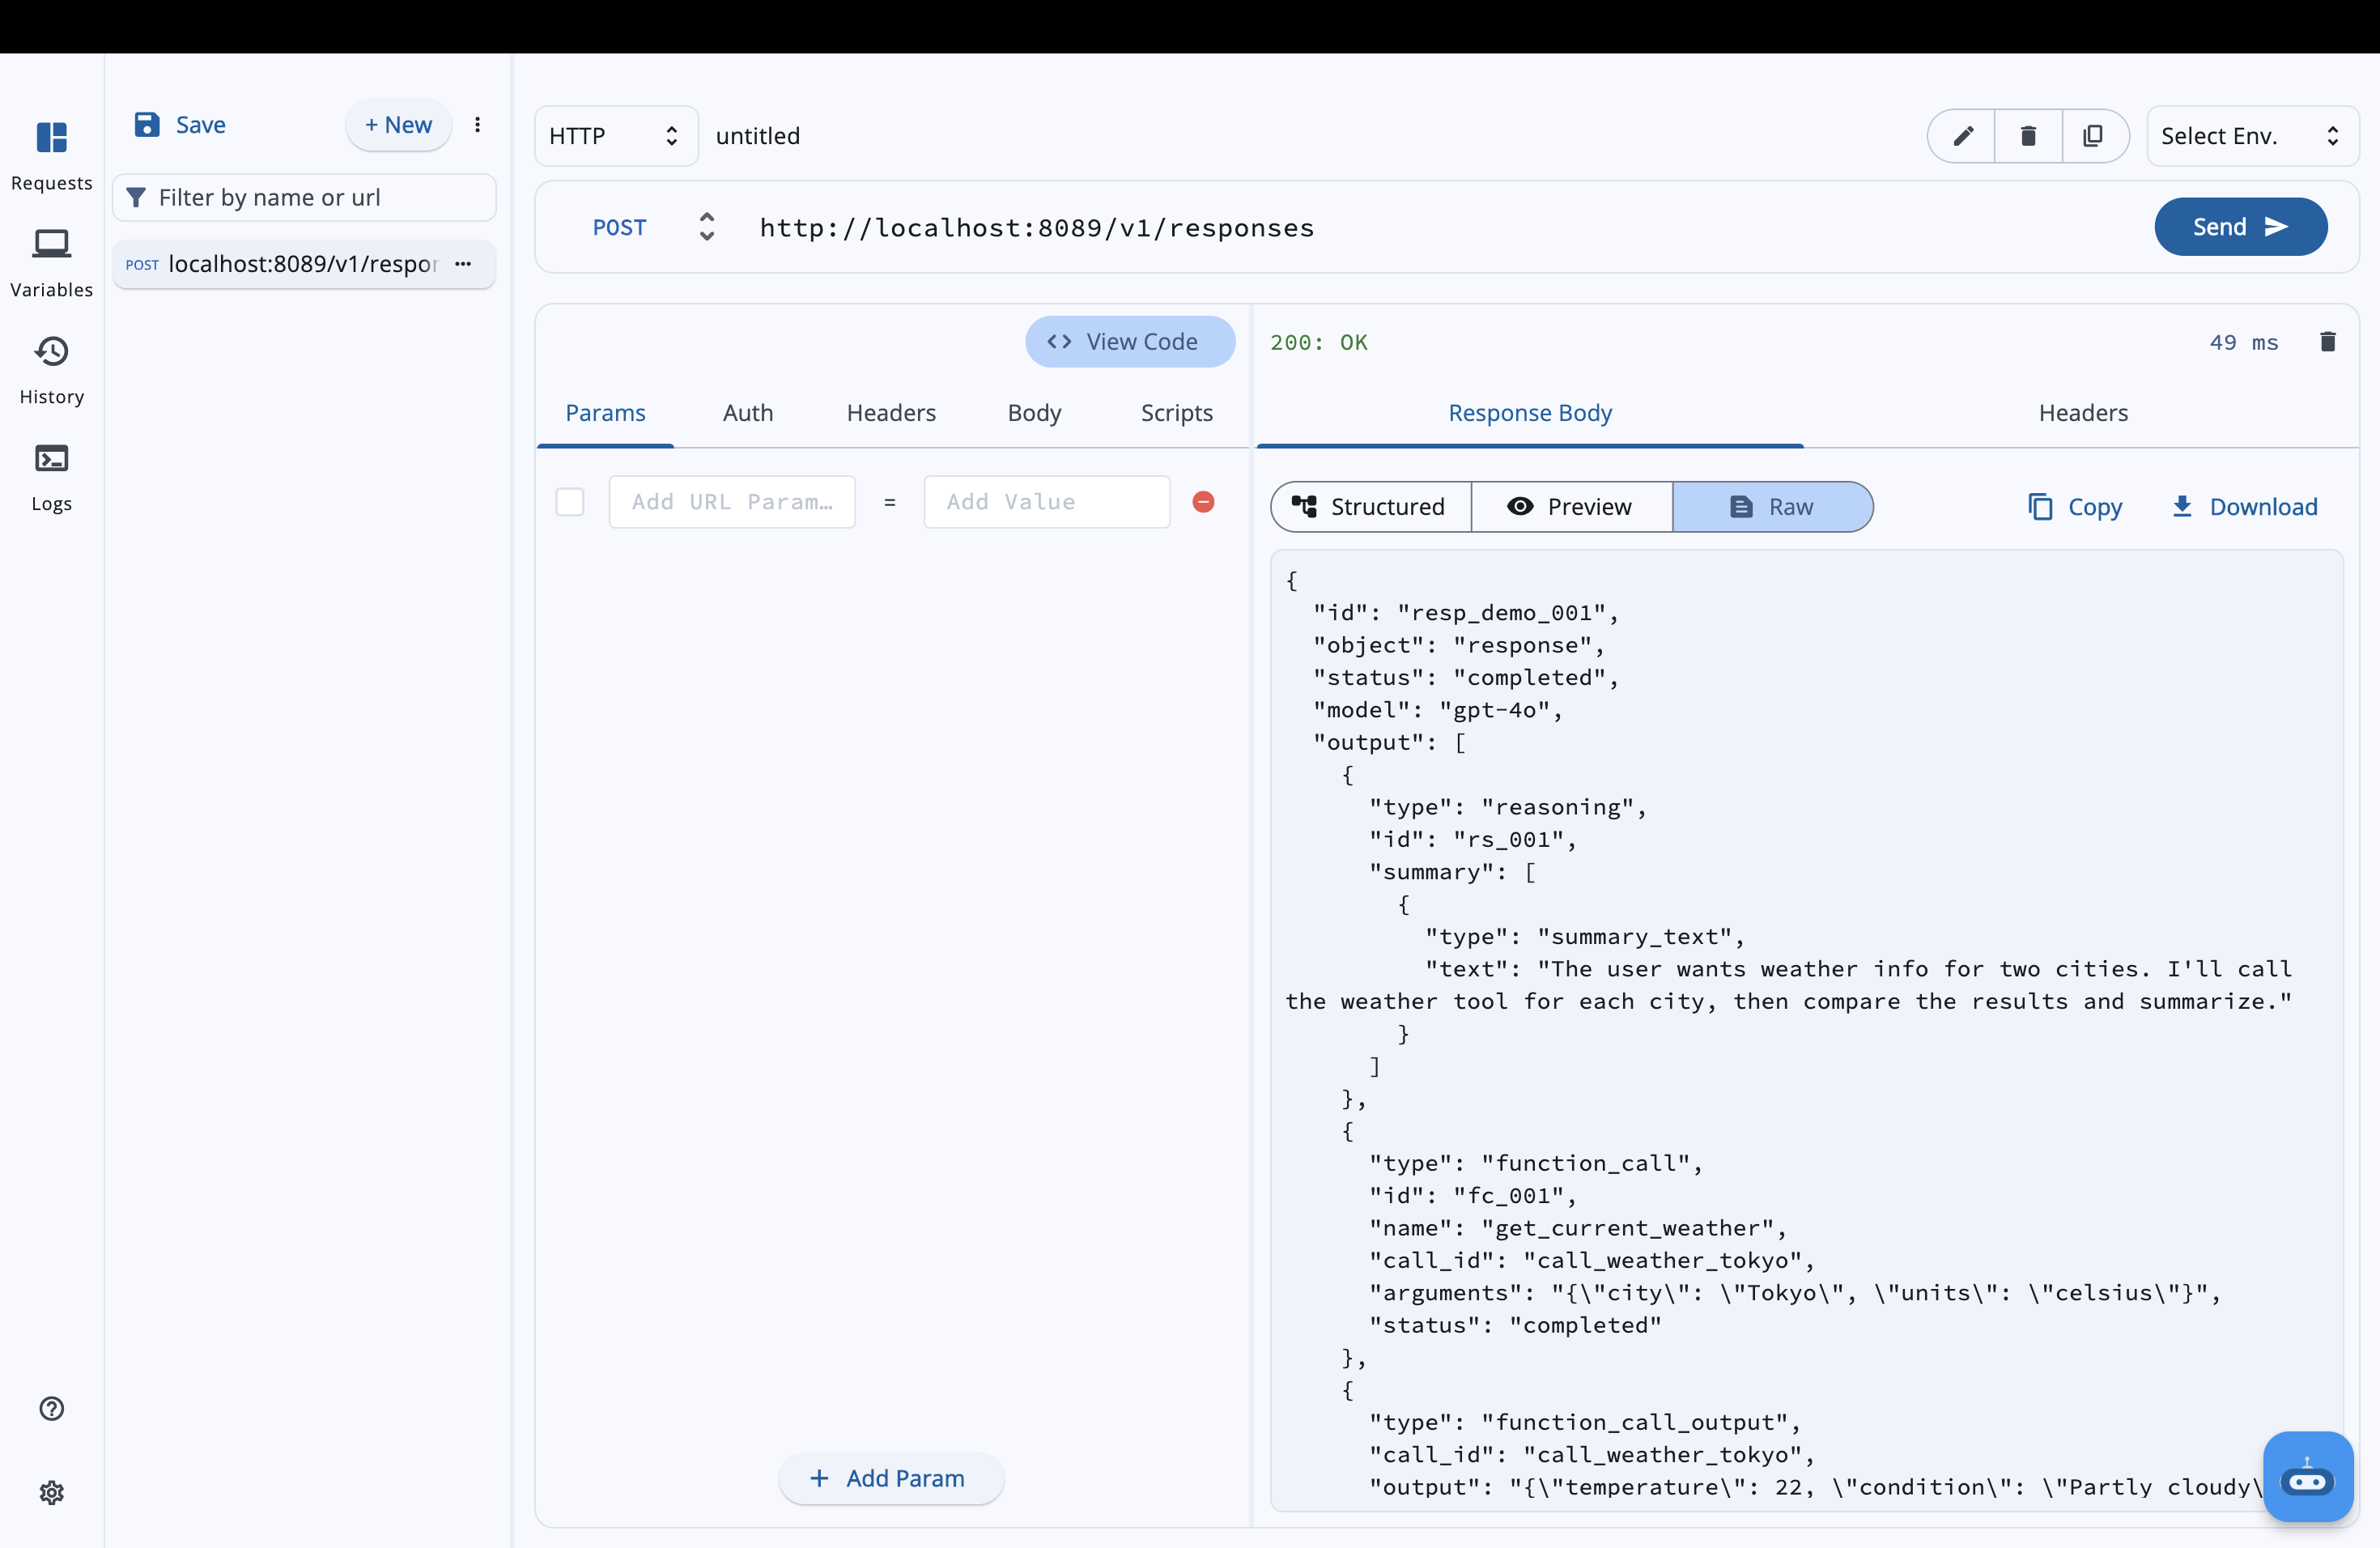
\includegraphics[width=\dimexpr\linewidth-2\fboxrule\relax]{doc/proposals/2026/gsoc/images/open_responses_raw_json.png}}\\[5pt]
  {\small\textit{Raw Open Responses JSON --- how every tool shows it today}}
\end{minipage}
\hfill
\begin{minipage}[t]{0.485\textwidth}
  \centering
  \fbox{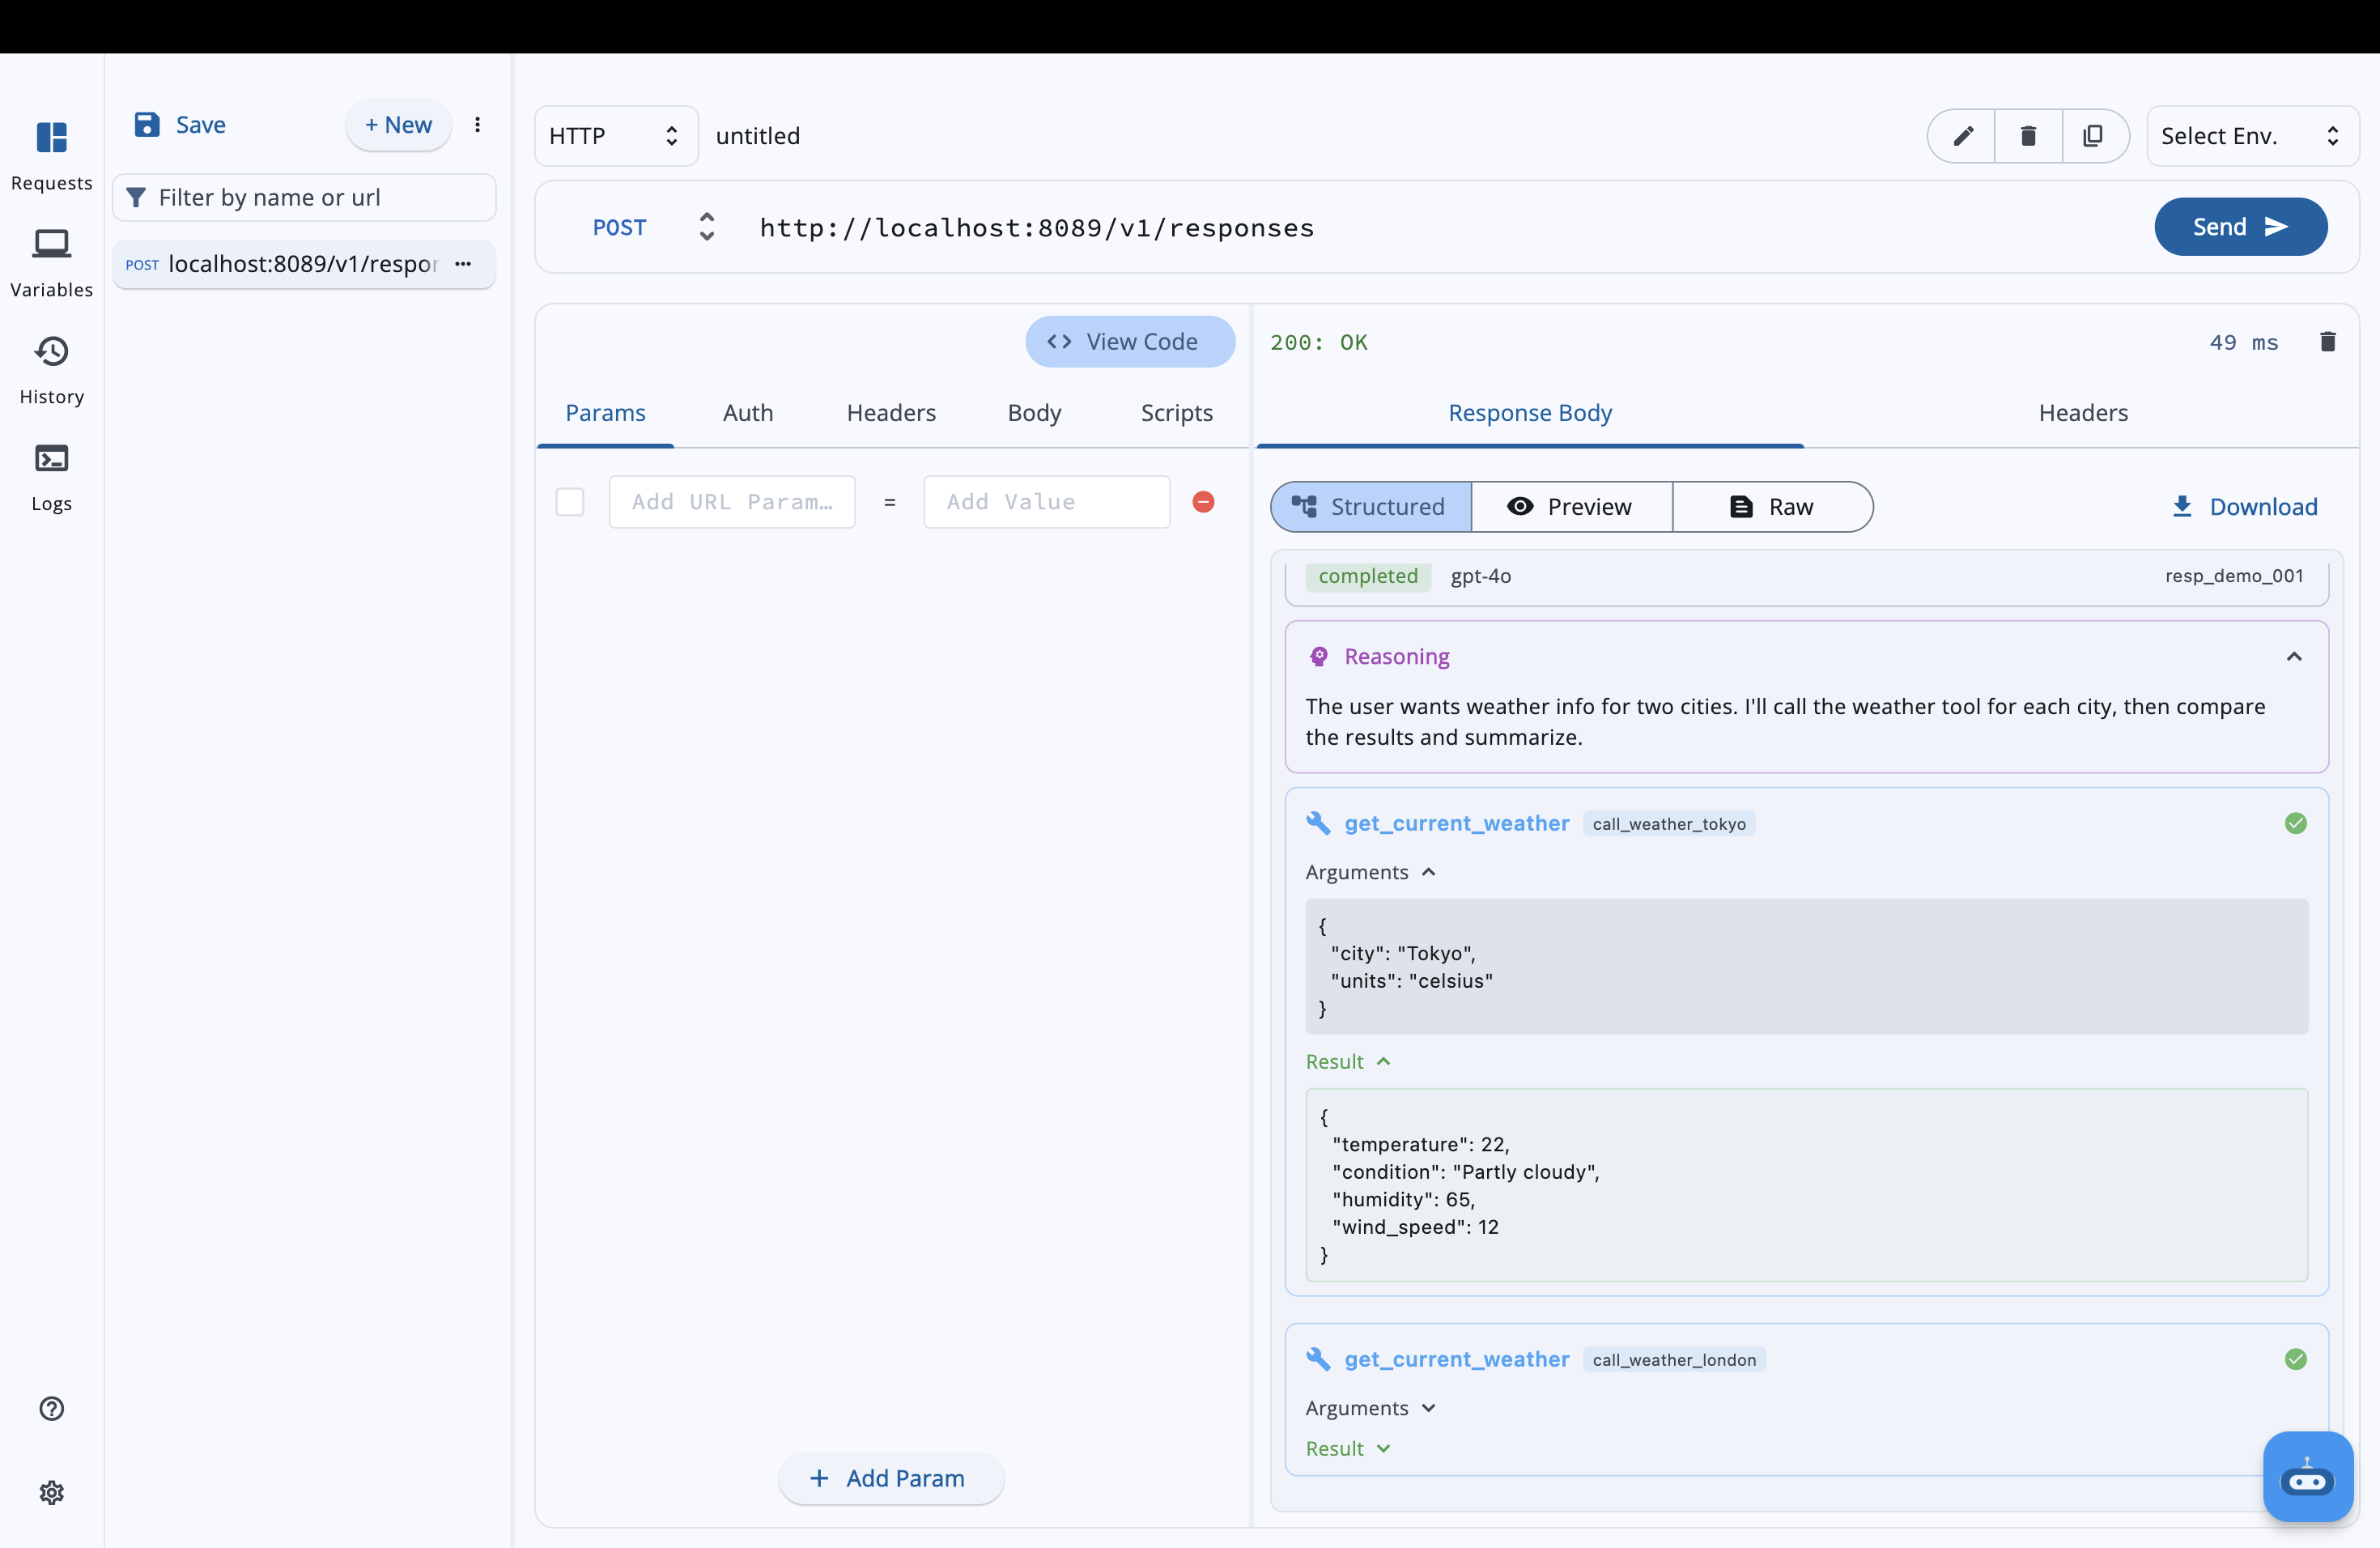
\includegraphics[width=\dimexpr\linewidth-2\fboxrule\relax]{doc/proposals/2026/gsoc/images/open_responses_structured_view.png}}\\[5pt]
  {\small\textit{Early prototype: structured card view (reasoning, tool calls, results separated). Much more to be built during GSoC.}}
\end{minipage}%
}
\vspace{10pt}

\textbf{3. A2UI Component Renderer} (\texttt{lib/widgets/a2ui\_renderer.dart} -- \textcolor{headerblue}{\bfseries 349 lines})

A registry-based renderer that maps \href{https://github.com/google/A2UI}{A2UI} component type strings to Flutter widget builders. The \texttt{A2UIParser} class handles detection (\texttt{isA2UIPayload}) and parsing of A2UI JSONL payloads. The \texttt{A2UIRenderer} is a \texttt{StatefulWidget} with local form state management, supporting \textcolor{headerblue}{\bfseries 15 component types}:

\begin{itemize}
  \item \textbf{Layout:} Card, Row, Column, List, Tabs
  \item \textbf{Display:} Text (with h1/h2/h3/caption variants), Image, Icon, Divider
  \item \textbf{Input:} Button (primary/outlined/text variants), TextField, Checkbox, Switch
  \item \textbf{Feedback:} Progress (determinate/indeterminate), Chip
  \item \textbf{Data Binding:} JSON Pointer path resolution from the data model (e.g., \texttt{/user/name})
\end{itemize}

Interactive components (TextField, Checkbox, Switch) maintain local state. Buttons show snackbar with action name. Unknown component types fall back to an error card showing the type name, so the renderer degrades gracefully.

\vspace{8pt}
{\setlength{\fboxsep}{0pt}\setlength{\fboxrule}{0.4pt}%
\noindent
\begin{minipage}[t]{0.485\textwidth}
  \centering
  \fbox{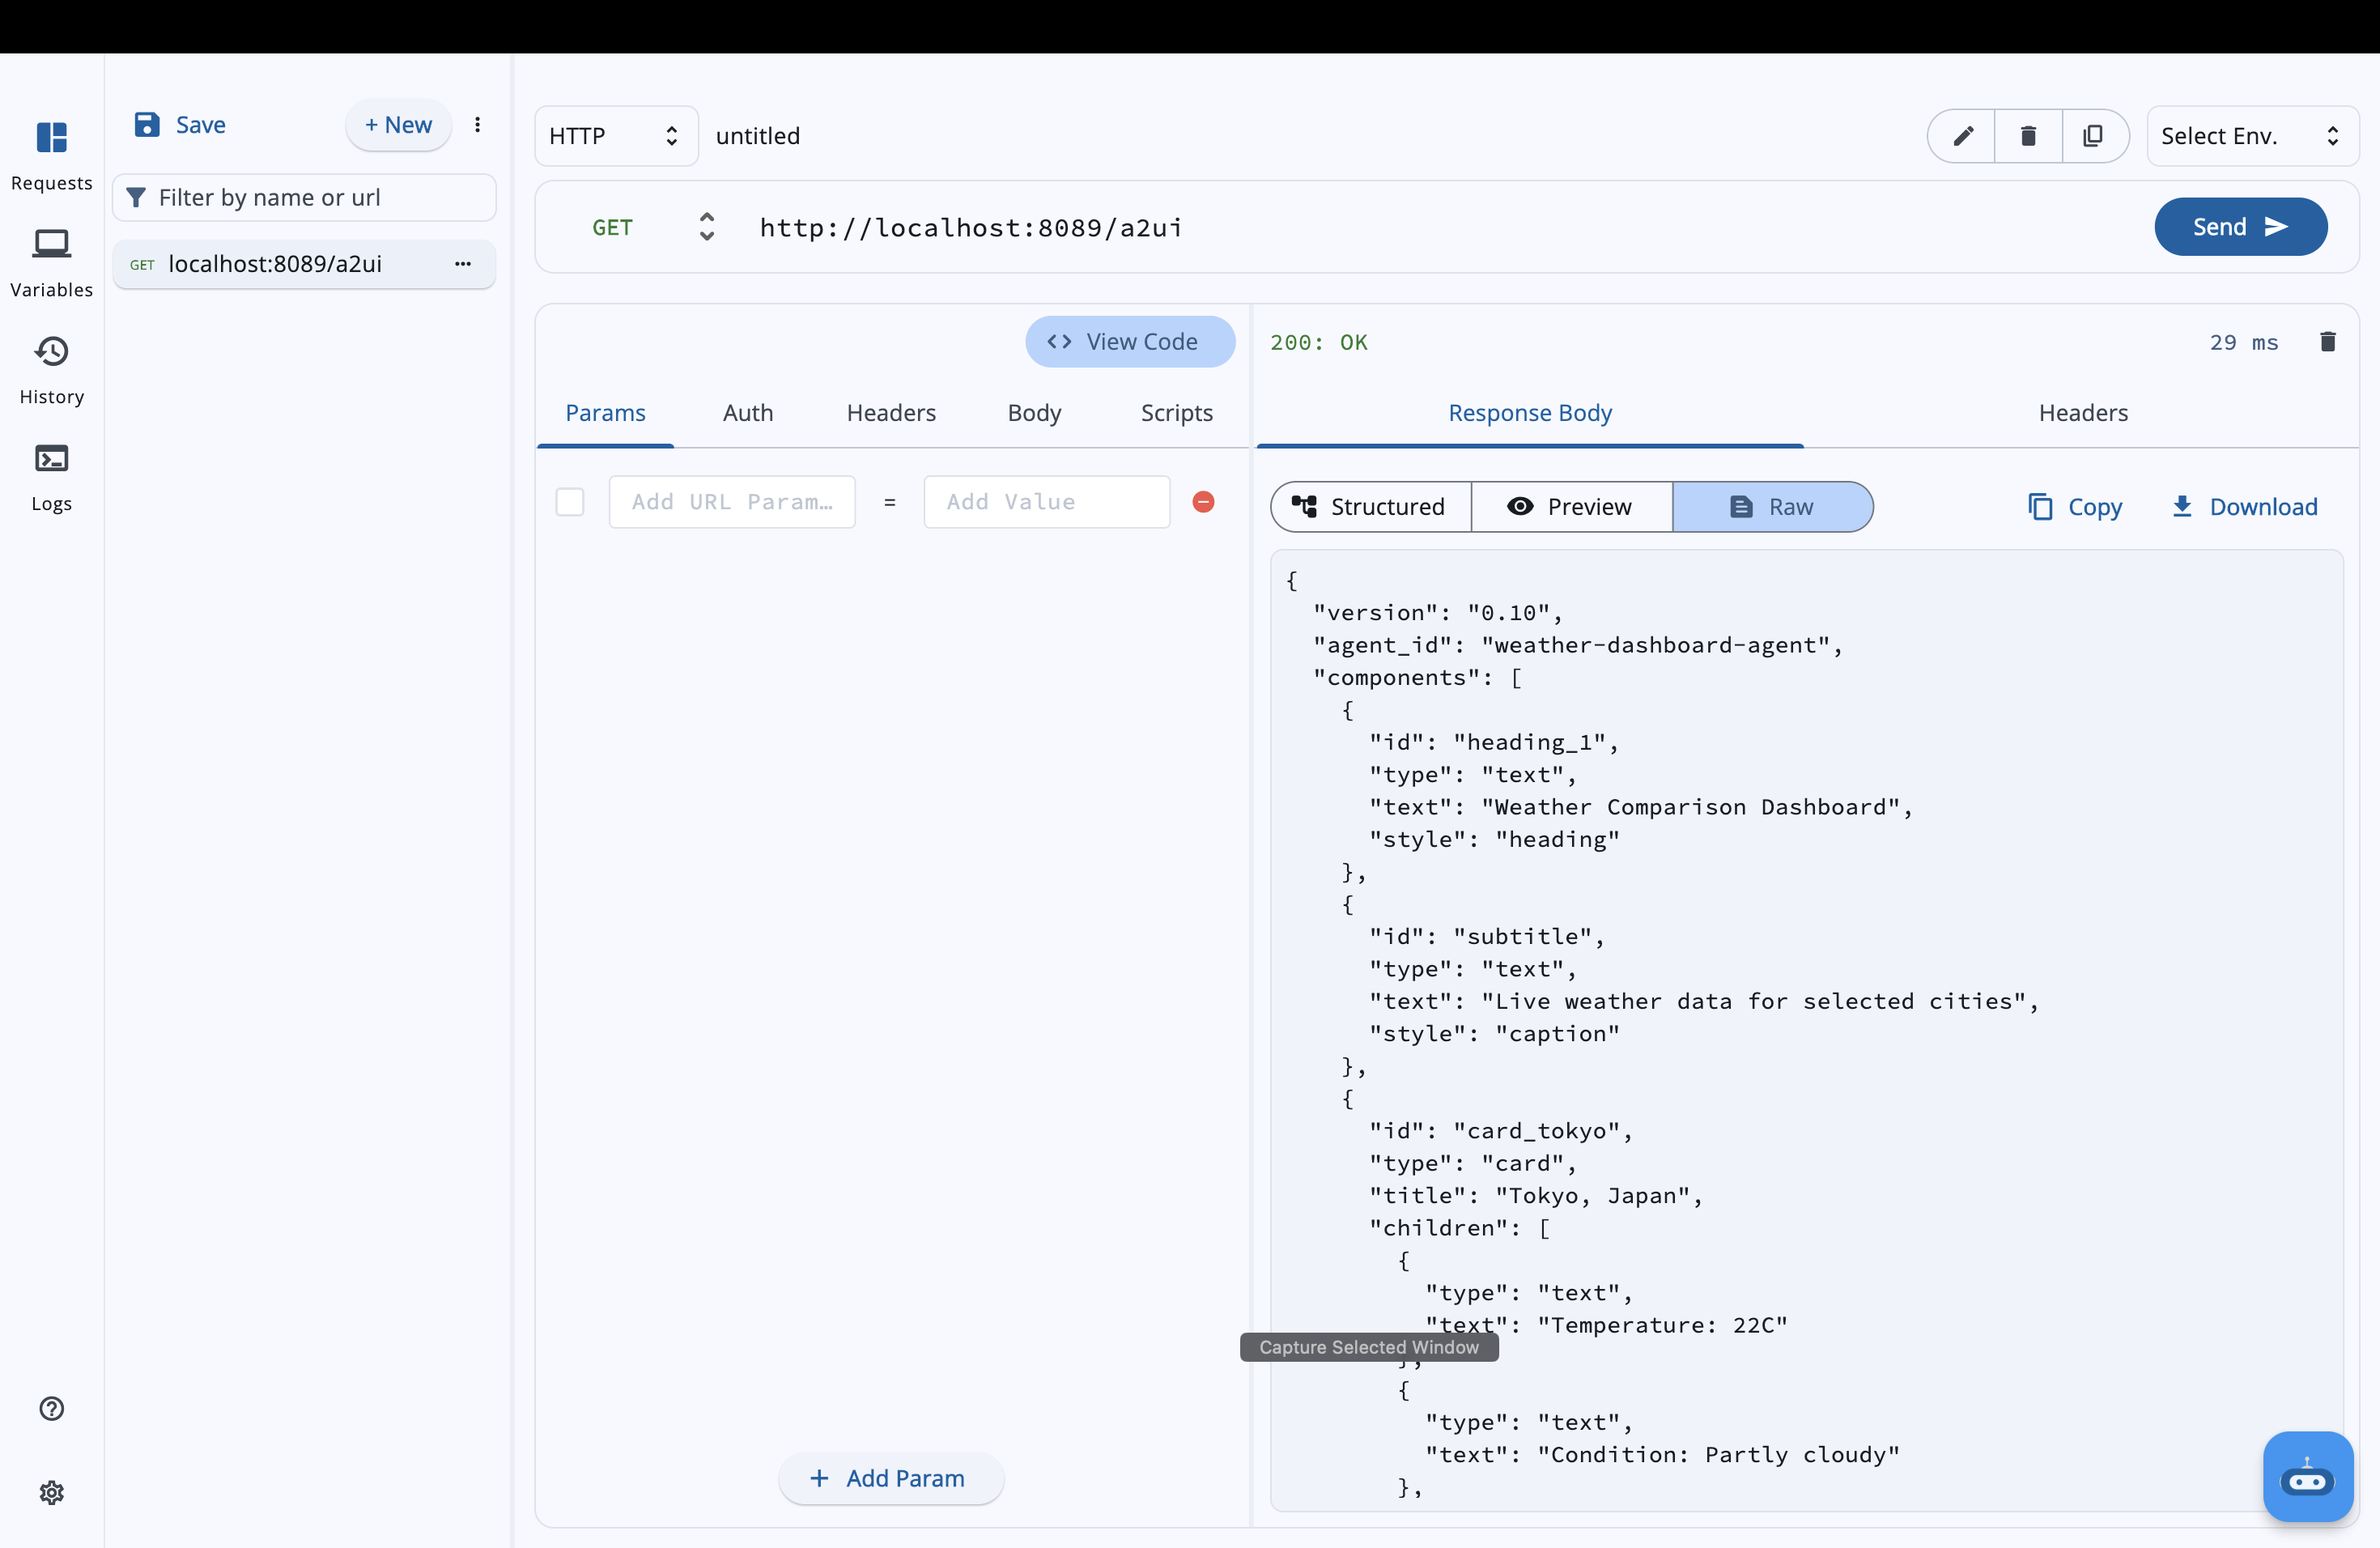
\includegraphics[width=\dimexpr\linewidth-2\fboxrule\relax]{doc/proposals/2026/gsoc/images/a2ui_raw_json.png}}\\[5pt]
  {\small\textit{A2UI component descriptors shown as raw JSON --- no tool renders this today}}
\end{minipage}
\hfill
\begin{minipage}[t]{0.485\textwidth}
  \centering
  \fbox{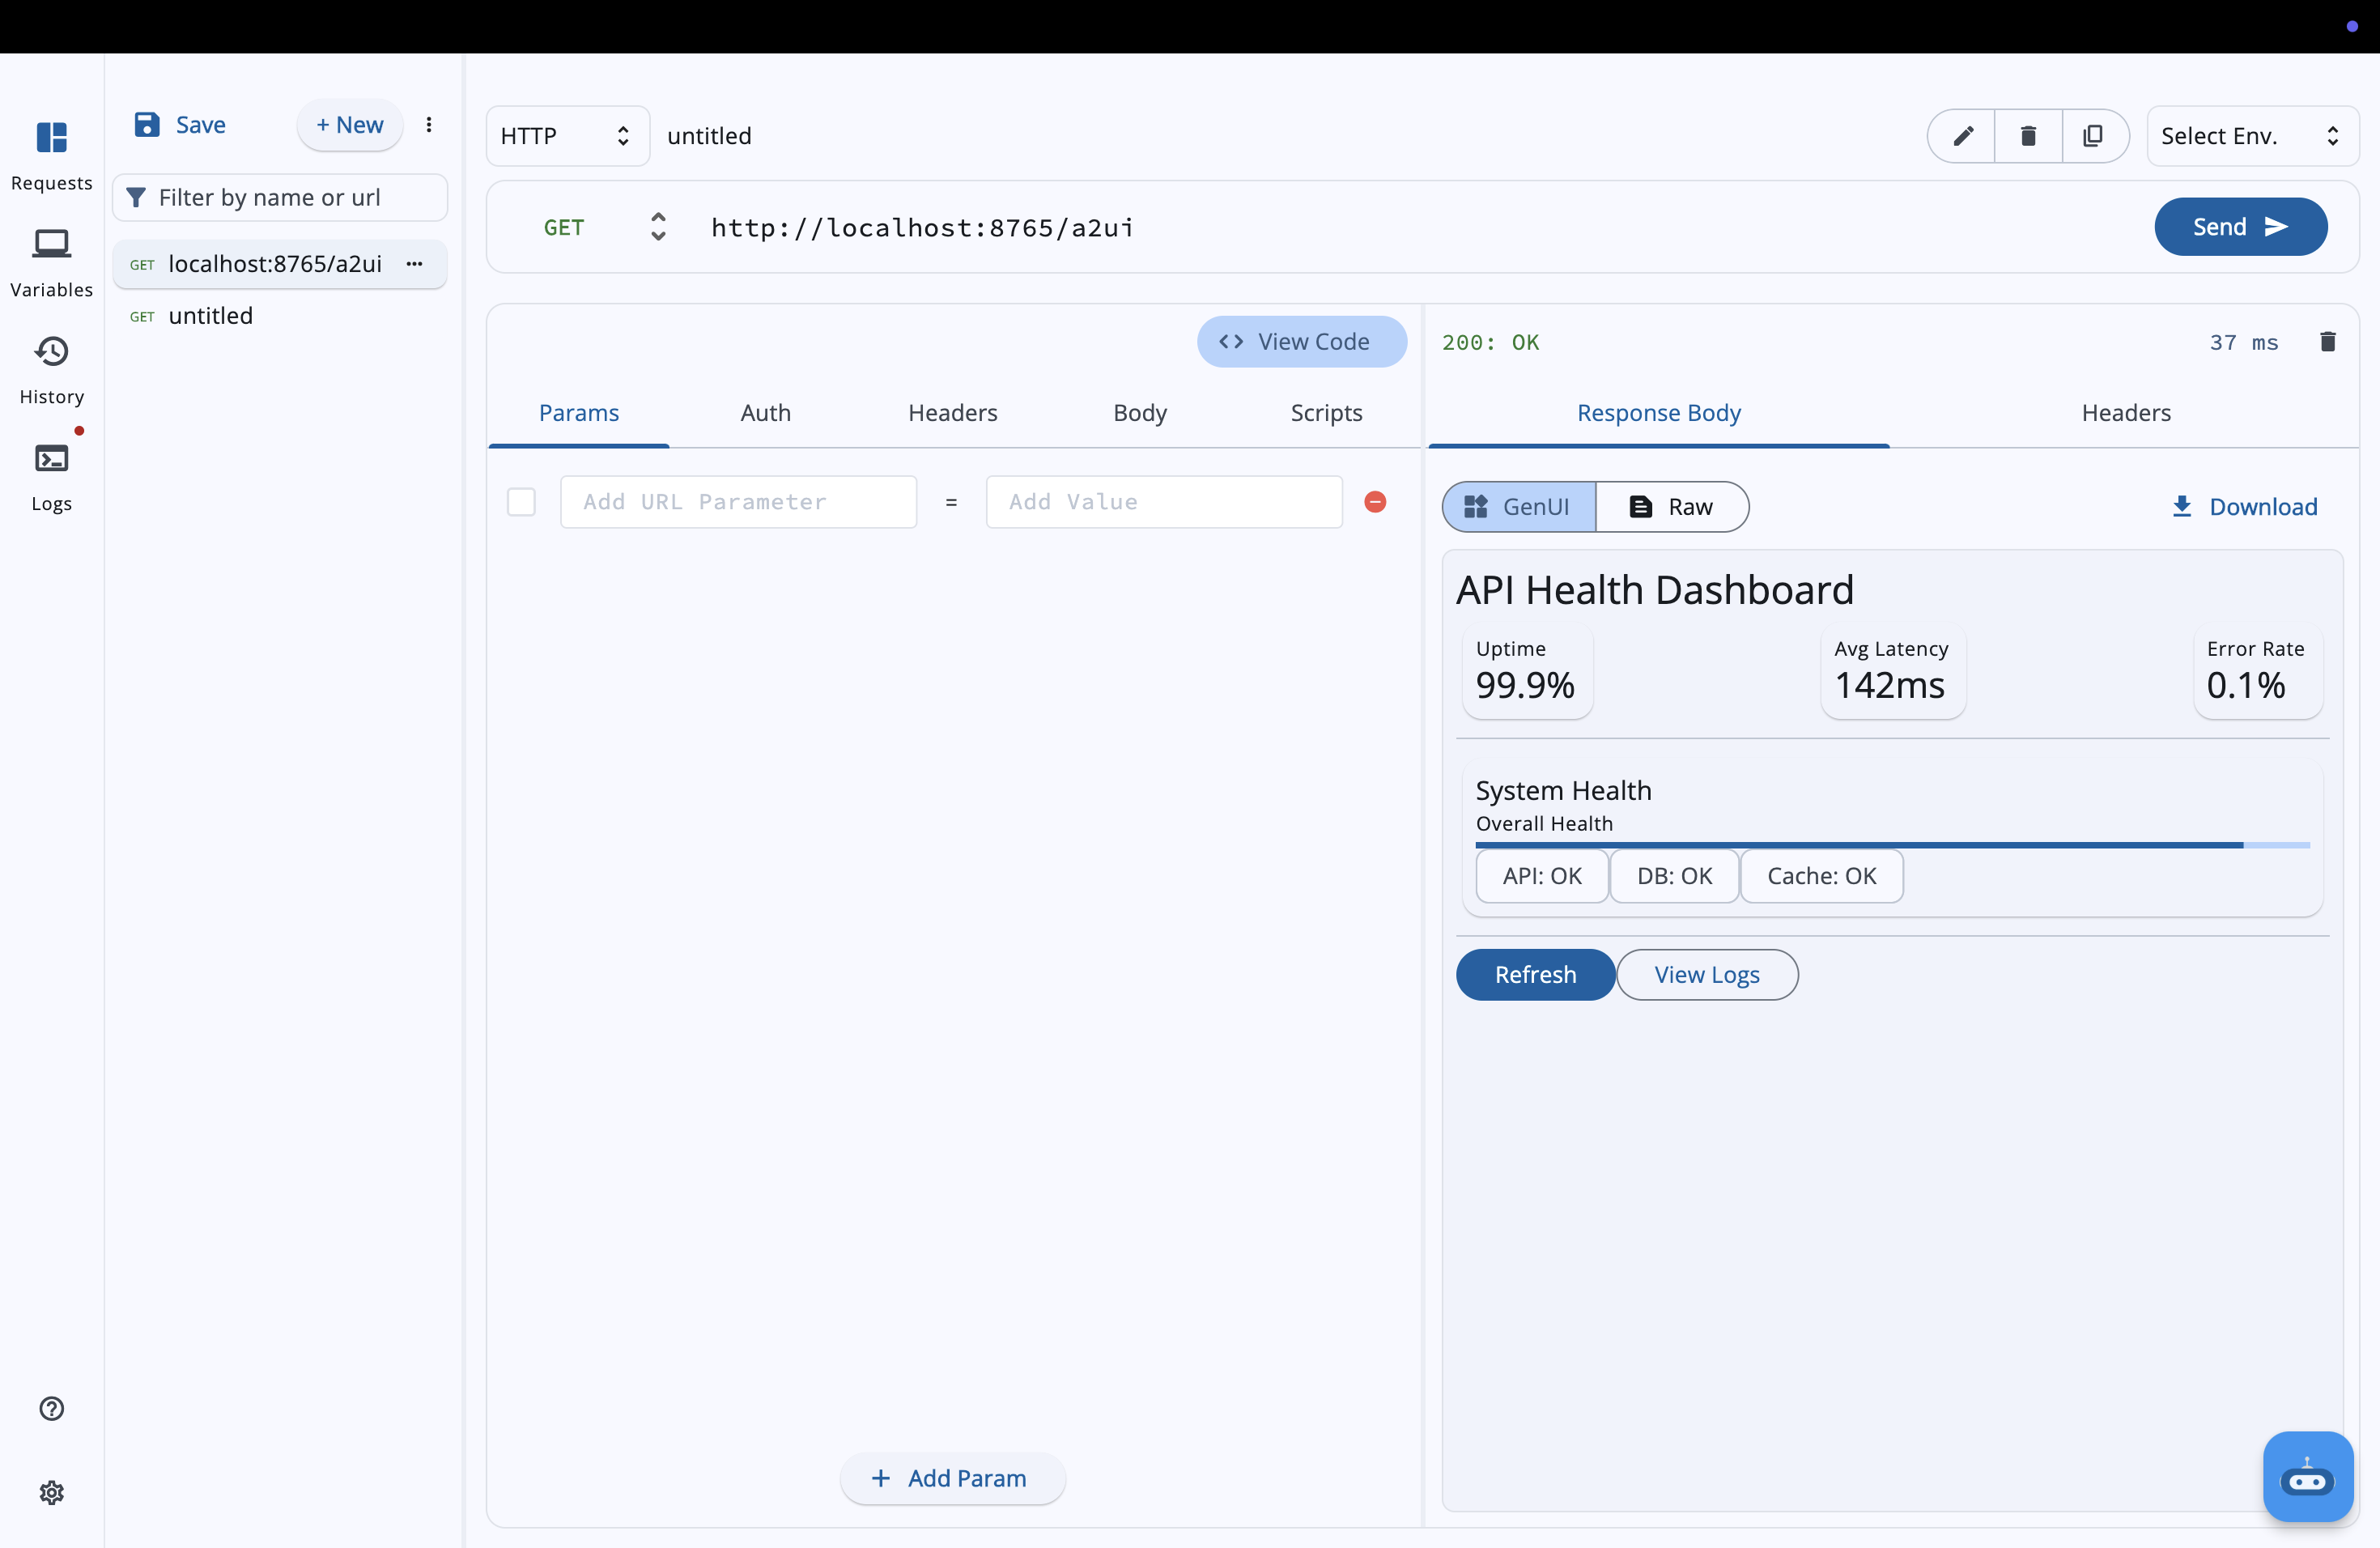
\includegraphics[width=\dimexpr\linewidth-2\fboxrule\relax]{doc/proposals/2026/gsoc/images/a2ui_rendered_dashboard.png}}\\[5pt]
  {\small\textit{Early prototype: same payload as a live interactive dashboard. Full A2UI spec coverage and streaming are planned for GSoC.}}
\end{minipage}%
}
\vspace{10pt}

\textbf{4. Response Pipeline Integration}

Extended the existing response pipeline with:

\begin{sloppypar}
\begin{itemize}
  \item Two new \texttt{ResponseBodyView} options: \texttt{structured} (for Open Responses) and \texttt{genui} (for A2UI).
  \item Auto-detection logic in \texttt{\_resolveViewOptions()} that checks for Open Responses format (\texttt{object == "response"} + \texttt{output[]} array) and A2UI format (\texttt{createSurface}/\texttt{updateComponents} keys).
  \item Routing to the appropriate viewer in \texttt{ResponseBodySuccess}.
\end{itemize}
\end{sloppypar}

\newpage

% ══════════════════════════════════════════════════════════════════════════════
%  TECHNICAL APPROACH
% ══════════════════════════════════════════════════════════════════════════════
\section{How I'll Build This -- Technical Approach for GSoC}

The PoC proves the concept works. But there's a meaningful gap between ``it works on fixture data'' and ``it handles real-world streaming responses with edge cases.'' Here's exactly how I plan to close that gap:

\subsection{A. Streaming with Typed SSE Events}

\begin{sloppypar}
\href{https://www.openresponses.org/}{Open Responses} streaming uses typed events like \texttt{response.output\_item.added}, \texttt{response.output\_text.delta}, \texttt{response.function\_call\_arguments.delta}, and \texttt{response.output\_item.done}. Each event targets a specific output item by index, so the parser needs to maintain a map of in-progress items and route deltas to the right place.
\end{sloppypar}

\begin{lstlisting}[style=darkcode]
class OpenResponsesStreamState {
    final List<OutputItem> items = [];
    final Map<int, StringBuffer> textBuffers = {};
    final Map<int, StringBuffer> argBuffers = {};

    void processEvent(String eventType,
        Map<String, dynamic> data) {
      switch (eventType) {
        case 'response.output_item.added':
          items.add(
            OutputItem.fromJson(data['item']));
        case 'response.output_text.delta':
          textBuffers[data['output_index']]?
            .write(data['delta']);
        case 'response.output_item.done':
          _finalizeItem(
            data['output_index'], data['item']);
      }
    }
}
\end{lstlisting}

\subsection{B. Conversation Chaining (\texttt{previous\_response\_id})}

Implementation plan:

\begin{itemize}
  \item Store \texttt{response.id} from each parsed response in the request model.
  \item Wire the stored ID into subsequent requests as \texttt{previous\_response\_id}.
  \item Build a timeline view that links related requests, showing the full conversation flow.
  \item Allow expanding/collapsing individual turns in the chain.
\end{itemize}

\subsection{C. Extended A2UI Component Support}

The PoC handles 15 component types with interactive state. The full implementation will expand this to cover the \href{https://github.com/google/A2UI}{A2UI specification} more completely:

\begin{itemize}
  \item \textbf{Input components:} TextField, DatePicker, Slider, Checkbox, Radio, Dropdown
  \item \textbf{Data display:} Table (with sorting/filtering), Progress bar, Charts (using \texttt{fl\_chart})
  \item \textbf{Navigation:} Tabs, Accordion, Stepper
  \item \textbf{Local state management:} Form state tracking, user interaction event logging
  \item \textbf{Progressive rendering:} Components render as they stream in via A2UI's flat ID-referenced model
\end{itemize}

\subsection{D. DashBot Integration}

Currently, DashBot renders all responses through \texttt{MarkdownBody} in \texttt{ChatBubble}. When DashBot's underlying AI provider returns an Open Responses format response, the integration would:

\begin{itemize}
  \item Parse the response using the same \texttt{OpenResponsesResult.fromJson} pipeline.
  \item Render structured output items inline in the chat (reasoning collapsed, tool calls as cards).
  \item If the response contains \href{https://github.com/google/A2UI}{A2UI} components, render them as interactive widgets within the chat bubble.
\end{itemize}

\subsection{Architecture Diagram}

\vspace{6pt}
\begin{center}
\resizebox{0.92\textwidth}{!}{%
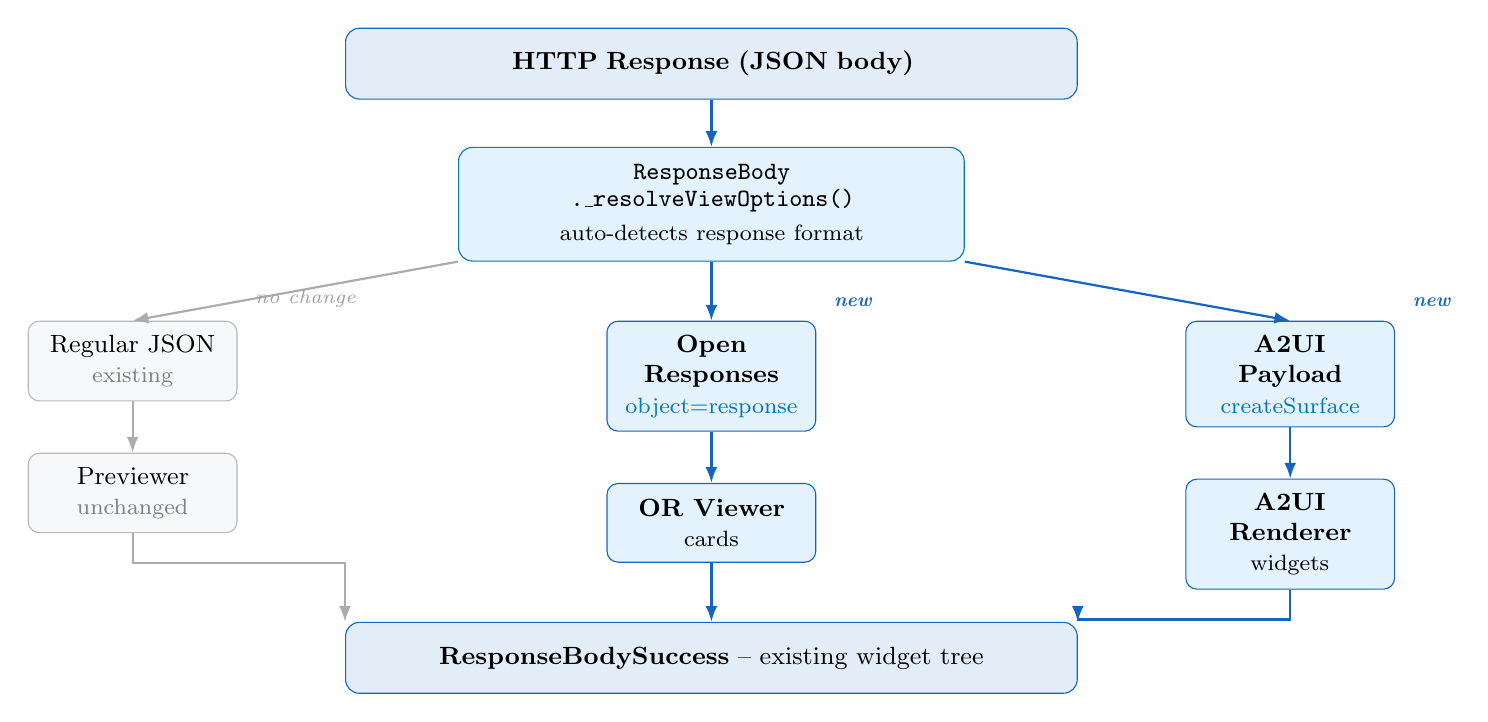
\begin{tikzpicture}[
  node distance=0.6cm and 0.5cm,
  topbox/.style={
    rectangle, rounded corners=5pt,
    draw=headerblue, fill=headerblue!12,
    text width=8.8cm, align=center,
    font=\small, inner sep=7pt, minimum height=0.9cm
  },
  detectbox/.style={
    rectangle, rounded corners=5pt,
    draw=subheadteal, fill=tblrowalt,
    text width=6cm, align=center,
    font=\small, inner sep=6pt, minimum height=0.9cm
  },
  existbox/.style={
    rectangle, rounded corners=4pt,
    draw=gray!55, fill=codebg,
    text width=2.3cm, align=center,
    font=\small, inner sep=5pt, minimum height=1cm
  },
  newbox/.style={
    rectangle, rounded corners=4pt,
    draw=headerblue, fill=tblrowalt,
    text width=2.3cm, align=center,
    font=\small\bfseries, inner sep=5pt, minimum height=1cm
  },
  arr/.style={-{Latex[length=2mm]}, thick, color=headerblue},
  garr/.style={-{Latex[length=2mm]}, thick, color=gray!65},
  lbl/.style={font=\scriptsize\itshape, color=gray!75, align=center}
]

\node[topbox] (http) {\textbf{HTTP Response (JSON body)}};

\node[detectbox, below=0.6cm of http] (detect)
  {\texttt{ResponseBody}\\[-1pt]\texttt{.\_resolveViewOptions()}\\[1pt]
   {\footnotesize\normalfont auto-detects response format}};

\draw[arr] (http) -- (detect);

\node[existbox, below left=0.75cm and 2.8cm of detect] (rjson)
  {Regular JSON\\{\footnotesize\color{gray}existing}};

\node[newbox, below=0.75cm of detect] (orresp)
  {Open Responses\\{\footnotesize\normalfont\color{subheadteal}object=response}};

\node[newbox, below right=0.75cm and 2.8cm of detect] (a2uip)
  {A2UI Payload\\{\footnotesize\normalfont\color{subheadteal}createSurface}};

\draw[garr] (detect.south west) -- (rjson.north);
\draw[arr]  (detect) -- (orresp);
\draw[arr]  (detect.south east) -- (a2uip.north);

\node[existbox, below=0.65cm of rjson] (prev)
  {Previewer\\{\footnotesize\color{gray}unchanged}};

\node[newbox, below=0.65cm of orresp] (orview)
  {OR Viewer\\{\footnotesize\normalfont cards}};

\node[newbox, below=0.65cm of a2uip] (a2uirend)
  {A2UI Renderer\\{\footnotesize\normalfont widgets}};

\draw[garr] (rjson) -- (prev);
\draw[arr]  (orresp) -- (orview);
\draw[arr]  (a2uip) -- (a2uirend);

\node[topbox, below=0.75cm of orview] (rbsuccess)
  {\textbf{ResponseBodySuccess} -- existing widget tree};

\draw[garr] (prev.south) |- ([yshift=-0.38cm]prev.south) -| (rbsuccess.north west);
\draw[arr]  (orview) -- (rbsuccess);
\draw[arr]  (a2uirend.south) |- ([yshift=-0.38cm]a2uirend.south) -| (rbsuccess.north east);

\node[lbl, above right=0.05cm and 0.1cm of rjson.north east] {no change};
\node[lbl, above right=0.05cm and 0.1cm of orresp.north east] {\textbf{\color{headerblue}new}};
\node[lbl, above right=0.05cm and 0.1cm of a2uip.north east] {\textbf{\color{headerblue}new}};

\end{tikzpicture}%
}% end resizebox
\end{center}
\vspace{4pt}

\subsection{What the End Result Will Look Like}

\textbf{Scenario 1 -- Testing an Open Responses endpoint (non-streaming):}

You send a request to an endpoint that follows the \href{https://www.openresponses.org/}{Open Responses protocol}. Instead of seeing a JSON blob, the response pane auto-switches to a structured view. You see the model's reasoning as a collapsed purple card at the top (click to expand the full chain-of-thought). Below that, tool calls show as blue cards -- each one shows the function name, a status chip, a pretty-printed version of the arguments, and the matching result right below it. The actual message text renders at the bottom as formatted markdown with inline images. A token usage bar at the bottom tells you how many tokens were used.

\textbf{Scenario 2 -- Streaming an agentic workflow:}

You send a streaming request. Cards appear one by one as the model generates output. First, a reasoning card pops up and its summary text fills in progressively. Then a function call card appears -- the function name shows immediately, and the arguments string grows character by character. When the tool result comes back, it slides in below the matching call. Finally, the message card appears and text streams into it. At no point do you see raw SSE events or JSON fragments.

\textbf{Scenario 3 -- Previewing an \href{https://github.com/google/A2UI}{A2UI} agent response:}

You send a request to a Vertex AI agent that returns A2UI component descriptors. Instead of seeing the JSON describing buttons, forms, and tables, you see actual rendered Flutter widgets -- interactive buttons you can tap, text fields you can type into, data tables with rows and columns. An event log panel shows what interactions the rendered UI generates, so you can verify your agent's UI behaves correctly.

\textbf{Scenario 4 -- Debugging a multi-turn agentic loop:}

You make three chained requests (each using \texttt{previous\_response\_id}). API Dash links them in a conversation timeline. You can see the full flow: first request $\to$ model reasons $\to$ calls tool A $\to$ you send result $\to$ model reasons again $\to$ calls tool B $\to$ you send result $\to$ model gives final answer. All in one connected view, not scattered across separate request tabs.

\subsection{What Could Go Wrong and How I'd Handle It}

\begin{center}
\begin{tabular}{|p{3.8cm}|p{1.8cm}|p{7.2cm}|}
\hline
\rowcolor{tblheader}
\textcolor{white}{\bfseries Risk} & \textcolor{white}{\bfseries Impact} & \textcolor{white}{\bfseries Mitigation} \\
\hline
\rowcolor{tblrowwhite}
Extending outputFormatter & High & Add a parallel \texttt{structuredOutputFormatter} path \\
\hline
\rowcolor{tblrowalt}
\href{https://github.com/google/A2UI}{A2UI} spec changes & Medium & Pin to specific version; unknown types show raw JSON \\
\hline
\rowcolor{tblrowwhite}
Streaming takes longer & Medium & Non-streaming structure works first as fallback \\
\hline
\rowcolor{tblrowalt}
Multi-turn chain state & Medium & Start with in-session track, persist later \\
\hline
\rowcolor{tblrowwhite}
Testing without API keys & Low & Already solved -- PoC includes fixture payloads \\
\hline
\end{tabular}
\end{center}

\newpage

% ══════════════════════════════════════════════════════════════════════════════
%  WEEKLY TIMELINE
% ══════════════════════════════════════════════════════════════════════════════
\section{Implementation Plan}

\textbf{Project Size:} 175 hours over 12 weeks ($\sim$15 hours/week)

\subsection{Community Bonding Period (May 8 -- June 1)}

\begin{itemize}
  \item Attend \href{https://lu.ma/calendar/cal-ZTW02O2EsWRs6V4}{weekly mentor sync-ups} and get feedback on the \href{https://github.com/foss42/apidash/pull/1358}{PoC}.
  \item Address any review comments on \href{https://github.com/foss42/apidash/pull/1321}{PR \#1321} (idea doc) and the PoC PR.
  \item Finalize design decisions with mentors: how to extend the provider interface for structured output, where to store conversation chain state, and the DashBot integration approach.
  \item Set up test fixtures for all edge cases (malformed responses, partial data, unknown output types).
\end{itemize}

\subsection{Phase 1 -- Open Responses Production Parser \& Structured Viewer (Weeks 1--3)}

\textcolor{subheadteal}{\bfseries Goal:} Turn the PoC's parsing and rendering into production-quality code.

\textbf{Week 1 (June 2 -- June 8)}
\begin{itemize}
  \item Finalize the \texttt{OpenResponsesResult} data models based on mentor feedback.
  \item Add handling for \texttt{output\_image} and \texttt{output\_file} content parts (PoC only handles \texttt{output\_text} and refusal).
  \item Implement robust format auto-detection with zero false positives on non-AI responses.
  \item Write unit tests for all \texttt{fromJson} factories using fixture payloads.
\end{itemize}
\deliverable{Production-ready \href{https://www.openresponses.org/}{Open Responses} parser in \texttt{packages/genai} with full test coverage.}

\textbf{Week 2 (June 9 -- June 15)}
\begin{itemize}
  \item Polish the Structured Response Viewer widgets (reasoning, function call, message cards).
  \item Add markdown rendering for message text content (using existing \texttt{flutter\_markdown} integration).
  \item Implement inline image rendering for \texttt{output\_image} parts (using existing \texttt{Image.memory}).
  \item Add a download button for \texttt{output\_file} parts.
\end{itemize}
\deliverable{Complete structured viewer rendering all Open Responses output types.}

\textbf{Week 3 (June 16 -- June 22)}
\begin{itemize}
  \item Wire the \texttt{OpenResponsesModel} provider into \texttt{kModelProvidersMap}.
  \item Implement \texttt{createRequest()} for the Responses API format (input + instructions).
  \item Implement non-streaming \texttt{outputFormatter} and \texttt{structuredOutputFormatter}.
  \item Integration tests: send requests via UI, verify auto-detection and structured rendering.
\end{itemize}
\deliverable{Working end-to-end flow -- user sees structured cards instead of raw JSON.}

\subsection{Phase 2 -- Streaming \& Conversation Chaining (Weeks 4--6)}

\textcolor{subheadteal}{\bfseries Goal:} Handle real-time streaming responses and multi-turn agentic workflows.

\textbf{Week 4 (June 23 -- June 29)}
\begin{itemize}
  \item Build the \texttt{OpenResponsesStreamState} machine for typed SSE events.
  \item Handle core event types:
    \begin{itemize}[nosep,topsep=1pt,leftmargin=2em]
      \item \texttt{response.output\_item.added}
      \item \texttt{response.output\_text.delta}
      \item \texttt{response.function\_call\_arguments.delta}
      \item \texttt{response.output\_item.done}
    \end{itemize}
  \item Wire stream state into \texttt{streamOutputFormatter} for the Open Responses provider.
\end{itemize}
\deliverable{Streaming parser that correctly routes typed deltas to output items.}

\textbf{Week 5 (June 30 -- July 6)}
\begin{itemize}
  \item Connect the stream state machine to the structured viewer for progressive rendering.
  \item Each output item card appears as \texttt{output\_item.added} fires; text and arguments fill in as deltas arrive.
  \item Handle edge cases: out-of-order events, partial data, connection drops.
  \item Write tests with recorded SSE fixtures.
\end{itemize}
\deliverable{Live streaming structured view -- cards build up in real-time.}

\textbf{Week 6 (July 7 -- July 13)}
\begin{itemize}
  \item Implement \texttt{previous\_response\_id} tracking in the request model.
  \item Build the conversation timeline view linking related requests.
  \item Allow expanding/collapsing individual turns in the chain.
  \item Mentor review before midterm evaluation.
\end{itemize}
\deliverable{Multi-turn conversation chaining with a connected timeline view.}

\textbf{Midterm Evaluation (July 14 -- July 18)}

{\setlength{\fboxsep}{9pt}%
\noindent\colorbox{green!10}{%
  \parbox{\dimexpr\linewidth-2\fboxsep\relax}{%
    \vspace{2pt}%
    {\small\textcolor{green!45!black}{\bfseries Expected state:} Full Open Responses support (parsing, structured viewing, streaming, conversation chaining) working end-to-end.}%
    \vspace{2pt}%
  }%
}}%

\subsection{Phase 3 -- A2UI Component Renderer (Weeks 7--9)}

\textcolor{subheadteal}{\bfseries Goal:} Extend the PoC's \href{https://github.com/google/A2UI}{A2UI} renderer to cover the full spec with interactive state and event logging.

\textbf{Week 7 (July 21 -- July 27)}
\begin{itemize}
  \item Expand the component registry to cover all core A2UI types: TextField, DatePicker, Slider, Checkbox, Radio, Dropdown, Table, Progress, Accordion, Stepper.
  \item Implement data binding resolution for all input types.
  \item Add local form state management.
\end{itemize}
\deliverable{\href{https://github.com/google/A2UI}{A2UI} renderer supporting \textcolor{headerblue}{\bfseries 20+} component types with interactive state.}

\textbf{Week 8 (July 28 -- August 3)}
\begin{itemize}
  \item Implement event logging system: user interactions with rendered components are captured in a collapsible log panel.
  \item Add progressive rendering: components render as they stream in via \texttt{updateComponents}.
  \item Handle component updates by ID (agents can update individual components).
\end{itemize}
\deliverable{Interactive A2UI renderer with event logging and progressive rendering.}

\textbf{Week 9 (August 4 -- August 10)}
\begin{itemize}
  \item Build the A2UI detection and routing pipeline (extending \texttt{\_resolveViewOptions()}).
  \item Add support for mixed responses (Open Responses output containing A2UI component descriptors).
  \item Write comprehensive tests for component rendering with various payloads.
  \item Mentor review.
\end{itemize}
\deliverable{Full \href{https://github.com/google/A2UI}{A2UI} rendering pipeline integrated into the response viewer.}

\subsection{Phase 4 -- DashBot Integration \& Polish (Weeks 10--12)}

\textcolor{subheadteal}{\bfseries Goal:} Bring structured AI responses into DashBot and polish everything for merge.

\textbf{Week 10 (August 11 -- August 17)}
\begin{itemize}
  \item Extend \texttt{ChatBubble} in DashBot to render structured Open Responses output inline.
  \item When DashBot receives a response with reasoning/tool calls, render them as cards within the chat.
  \item Add A2UI component rendering within chat bubbles for interactive agent responses.
\end{itemize}
\deliverable{DashBot with rich structured response rendering.}

\textbf{Week 11 (August 18 -- August 24)}
\begin{itemize}
  \item End-to-end testing with real API endpoints (OpenAI Responses API, compatible providers).
  \item Edge case handling: malformed responses, partial streams, mixed content types, very large responses.
  \item Performance profiling: ensure structured rendering does not add noticeable latency.
  \item Fix bugs identified during testing.
\end{itemize}
\deliverable{Battle-tested implementation passing all edge cases.}

\textbf{Week 12 (August 25 -- September 1)}
\begin{itemize}
  \item Code cleanup, documentation, and final polish.
  \item Ensure all new code follows API Dash's existing patterns and conventions.
  \item Write developer documentation for extending the component registry.
  \item Final mentor review and project report.
\end{itemize}
\deliverable{Merge-ready code with documentation.}

{\setlength{\fboxsep}{12pt}\setlength{\fboxrule}{1pt}%
\noindent\fcolorbox{stretchborder}{stretchbg}{%
  \parbox{\dimexpr\textwidth-2\fboxsep-2\fboxrule\relax}{%
    \vspace{2pt}%
    {\small\bfseries\color{stretchborder}$\star$\enspace Stretch Goals (if time permits)}%
    \vspace{6pt}\par
    \begin{itemize}[topsep=0pt,itemsep=4pt]
      \item \textbf{A2UI Live Playground:} A split-pane editor where you can edit A2UI JSON on the left and see rendered Flutter widgets update on the right in real-time.
      \item \textbf{Visual Conversation Debugger:} An enhanced multi-turn view with collapsible branches, search/filter by output type, and export of full conversation chains as shareable reports.
    \end{itemize}%
    \vspace{2pt}%
  }%
}}%

\newpage

% ══════════════════════════════════════════════════════════════════════════════
%  CONTRIBUTIONS
% ══════════════════════════════════════════════════════════════════════════════
\section{Contributions to API Dash}

\begin{center}
\begin{tabular}{|p{1.8cm}|p{9cm}|p{2cm}|}
\hline
\rowcolor{tblheader}
\textcolor{white}{\bfseries PR} & \textcolor{white}{\bfseries Description} & \textcolor{white}{\bfseries Status} \\
\hline
\rowcolor{tblrowwhite}
\href{https://github.com/foss42/apidash/pull/1279}{\#1279}
  & Input validation for empty API key and endpoint URL in AI Model Selector dialog
  & \cellcolor{orange!10}\textcolor{orange!65!black}{\bfseries Open} \\
\hline
\rowcolor{tblrowalt}
\href{https://github.com/foss42/apidash/pull/1290}{\#1290}
  & Custom OpenAI-compatible LLM provider support (Groq, OpenRouter, Mistral, etc.)
  & \cellcolor{orange!10}\textcolor{orange!65!black}{\bfseries Open} \\
\hline
\rowcolor{tblrowwhite}
\href{https://github.com/foss42/apidash/pull/1321}{\#1321}
  & GSoC 2026 idea doc -- Open Responses \& Generative UI
  & \cellcolor{green!12}\textcolor{green!45!black}{\bfseries Merged} \\
\hline
\rowcolor{tblrowalt}
\href{https://github.com/foss42/apidash/pull/1358}{\#1358}
  & PoC -- Open Responses structured viewer + A2UI component renderer
    (\href{https://youtu.be/paN-KGIhNms}{demo 1},
     \href{https://youtu.be/T2KbHth736U}{demo 2})
  & \cellcolor{orange!10}\textcolor{orange!65!black}{\bfseries Open} \\
\hline
\end{tabular}
\end{center}

\section{Contributions to Other Open-Source Projects}

\textbf{astropy -- Python, 500k+ lines, widely used astronomy library}

\begin{center}
\begin{tabular}{|p{1.8cm}|p{9cm}|p{2cm}|}
\hline
\rowcolor{tblheader}
\textcolor{white}{\bfseries PR} & \textcolor{white}{\bfseries Description} & \textcolor{white}{\bfseries Status} \\
\hline
\rowcolor{tblrowwhite}
\href{https://github.com/astropy/astropy/pull/19403}{\#19403}
  & Fixed missing f-string prefix in \texttt{BaseAffineTransform.\_apply\_transform}
  & \cellcolor{green!12}\textcolor{green!45!black}{\bfseries Merged} \\
\hline
\rowcolor{tblrowalt}
\href{https://github.com/astropy/astropy/pull/19404}{\#19404}
  & Fixed silent data corruption in \texttt{FITS\_rec} slice assignment with negative indices
  & \cellcolor{green!12}\textcolor{green!45!black}{\bfseries Merged} \\
\hline
\rowcolor{tblrowwhite}
\href{https://github.com/astropy/astropy/pull/19450}{\#19450}
  & Fixed table index corruption when a row assignment fails
  & \cellcolor{green!12}\textcolor{green!45!black}{\bfseries Merged} \\
\hline
\end{tabular}
\end{center}

\vspace{8pt}
\textbf{Hyperledger Besu -- Java, Ethereum execution client}

\begin{center}
\begin{tabular}{|p{1.8cm}|p{9cm}|p{2cm}|}
\hline
\rowcolor{tblheader}
\textcolor{white}{\bfseries PR} & \textcolor{white}{\bfseries Description} & \textcolor{white}{\bfseries Status} \\
\hline
\rowcolor{tblrowwhite}
\href{https://github.com/hyperledger/besu/pull/10020}{\#10020}
  & Fixed critical bug where \texttt{serializeAndDedupOperation()} never returned \texttt{failedFuture}
  & \cellcolor{green!12}\textcolor{green!45!black}{\bfseries Merged} \\
\hline
\rowcolor{tblrowalt}
\href{https://github.com/hyperledger/besu/pull/10042}{\#10042}
  & Fixed \texttt{eth\_estimateGas} using parent block's hash instead of current block's hash
  & \cellcolor{green!12}\textcolor{green!45!black}{\bfseries Merged} \\
\hline
\rowcolor{tblrowwhite}
\href{https://github.com/hyperledger/besu/pull/10051}{\#10051}
  & Fixed TOCTOU race condition in \texttt{eth\_getBlockByNumber}
  & \cellcolor{green!12}\textcolor{green!45!black}{\bfseries Merged} \\
\hline
\rowcolor{tblrowalt}
\href{https://github.com/hyperledger/besu/pull/10060}{\#10060}
  & Fixed unsigned underflow in \texttt{eth\_feeHistory} reward bounds calculation
  & \cellcolor{green!12}\textcolor{green!45!black}{\bfseries Merged} \\
\hline
\end{tabular}
\end{center}

\vspace{8pt}
\textbf{Hyperledger Fabric -- Go, enterprise blockchain platform}

\begin{center}
\begin{tabular}{|p{1.8cm}|p{9cm}|p{2cm}|}
\hline
\rowcolor{tblheader}
\textcolor{white}{\bfseries PR} & \textcolor{white}{\bfseries Description} & \textcolor{white}{\bfseries Status} \\
\hline
\rowcolor{tblrowwhite}
\href{https://github.com/hyperledger/fabric/pull/5422}{\#5422}
  & Fixed gossip protocol not returning after sending NACK on private data store failure
  & \cellcolor{green!12}\textcolor{green!45!black}{\bfseries Merged} \\
\hline
\rowcolor{tblrowalt}
\href{https://github.com/hyperledger/fabric/pull/5424}{\#5424}
  & Fixed resource leak: \texttt{collItr} not being closed before releasing \texttt{purgerLock}
  & \cellcolor{green!12}\textcolor{green!45!black}{\bfseries Merged} \\
\hline
\rowcolor{tblrowwhite}
\href{https://github.com/hyperledger/fabric/pull/5430}{\#5430}
  & Fixed iterator leak in \texttt{deleteDataMarkedForPurge}
  & \cellcolor{green!12}\textcolor{green!45!black}{\bfseries Merged} \\
\hline
\end{tabular}
\end{center}

\vspace{8pt}
\textbf{LFDT-Lockness/generic-ec -- Rust, elliptic curve cryptography}

\begin{center}
\begin{tabular}{|p{1.8cm}|p{9cm}|p{2cm}|}
\hline
\rowcolor{tblheader}
\textcolor{white}{\bfseries PR} & \textcolor{white}{\bfseries Description} & \textcolor{white}{\bfseries Status} \\
\hline
\rowcolor{tblrowwhite}
\href{https://github.com/LFDT-Lockness/generic-ec/pull/59}{\#59}
  & Added secp384r1 (NIST P-384) curve support -- first non-32-byte scalar curve, 180 tests passing
  & \cellcolor{green!12}\textcolor{green!45!black}{\bfseries Merged} \\
\hline
\end{tabular}
\end{center}

\newpage

% ══════════════════════════════════════════════════════════════════════════════
%  WHY ME
% ══════════════════════════════════════════════════════════════════════════════
\section{Why Me}

{\setlength{\fboxsep}{10pt}%
\noindent\colorbox{tblrowalt}{%
  \parbox{\dimexpr\linewidth-2\fboxsep\relax}{%
    \centering\small
    \textcolor{headerblue}{\bfseries 5} open-source projects\enspace$\cdot$\enspace
    \textcolor{headerblue}{\bfseries 11} merged PRs\enspace$\cdot$\enspace
    \textcolor{headerblue}{\bfseries 4} API Dash PRs\enspace$\cdot$\enspace
    \textcolor{headerblue}{\bfseries $\sim$1{,}100} lines of working PoC
  }%
}}%
\vspace{10pt}

I'll be honest -- I'm a first-year student applying to work on something that matters to me, not just something that looks good on a resume. I've been genuinely frustrated with how every API tool handles AI responses. I tested Postman, Insomnia, Thunder Client with real agentic APIs -- and every single one just dumps the JSON. I kept thinking \textit{``there has to be a better way to see this.''} That frustration is what started all of this.

Before I wrote a single line of proposal text, I spent two weeks just reading the API Dash codebase. Not skimming -- actually reading. I traced how a raw HTTP response becomes a rendered widget. I read how \texttt{ModelProvider} abstracts different AI backends, how \texttt{ResponseBodyView} decides what to show, how the Stac pipeline connects provider output to the UI. It took a while, and I got lost more than once. But by the end of it I knew exactly where my code had to live -- not just where it would work, but where it \textit{belonged}.

Then I built the PoC. Not because the application required it, but because I genuinely wasn't sure I could do it -- and I needed to find out. The sealed class hierarchy, the widget tree, the A2UI registry, wiring it all into the existing pipeline without breaking anything -- \textcolor{headerblue}{\bfseries 1,100 lines} later, it works. There are still hard parts ahead (the streaming state machine, conversation chaining), but I now know the codebase well enough to know where those pieces go.

What I want to build isn't just a feature. It's something I'd use every day, and something every developer testing AI APIs would benefit from. That's not a pitch -- it's genuinely why I chose this project over everything else in the ideas list.

\label{docendpage}
\end{document}
